% Consolidated reference source for Andre Manada Correia da Silva, TALLY.
% Generated from Tally_André_Manada.zip / EstiloTeses on 2026-06-18.
% The original multi-file LaTeX source was flattened into this single file;
% all image assets live under ./images/.

% Document Type: LaTeX
% Master File: thesis.tex
\documentclass[12pt,a4paper]{report}
\usepackage[english]{babel}
\usepackage[utf8]{inputenc}
%\usepackage{epsf}             %incluir figuras encapsulated postscript
%\usepackage{amstex}          
%\pagestyle{myheadings}
\usepackage{changepage}
\usepackage{graphics}
\usepackage{csquotes}
\usepackage{textcmds}
\usepackage{graphicx}
\usepackage{multirow}
\usepackage{float}
\usepackage{todonotes}
% \usepackage{minted} % unused in this thesis source; left out to avoid requiring shell-escape
\usepackage{xcolor}
\usepackage{listings}
\usepackage{amsmath}
\usepackage{tikz}
\graphicspath{{images/}}

\definecolor{mGreen}{rgb}{0,0.6,0}
\definecolor{mGray}{rgb}{0.5,0.5,0.5}
\definecolor{mBlue}{rgb}{0.2,0.2,1}
\definecolor{mPurple}{rgb}{0.58,0,0.82}
\definecolor{mOrange}{rgb}{1,0.6,0.3}
\definecolor{backgroundColour}{rgb}{0.95,0.95,0.92}

\lstdefinestyle{CStyle}{
    backgroundcolor=\color{backgroundColour},   
    commentstyle=\color{mGreen},
    keywordstyle=\color{mBlue},
    numberstyle=\tiny\color{mGray},
    stringstyle=\color{mOrange},
    basicstyle=\footnotesize,
    breakatwhitespace=false,         
    breaklines=true,                 
    captionpos=b,                    
    keepspaces=true,                 
    numbers=left,                    
    numbersep=5pt,                  
    showspaces=false,                
    showstringspaces=false,
    showtabs=false,                  
    tabsize=2,
    language=C
}

\newenvironment{tightcenter}{%
  \setlength\topsep{0pt}
  \setlength\parskip{0pt}
  \begin{center}
}{%
  \end{center}
}

% -----------------------------------------------------------------------------
% Inlined FCUP thesis style from original fcthesis.sty.
% This keeps the reference source self-contained.
% -----------------------------------------------------------------------------
\makeatletter
% Versão para teses em inglês.
% Definicao do estilo da tese para o Dept. de CC da FCUP.
% Hacked from Manchester University thesis style (also hacked from 
% Stanford University thesis style suthesis.sty)
%
% 4/1991, Fernando: new commands added
%    \submitionplace{}, \department{} and \dedicationpage{},
%       now the cover page can be fully specified outside this style file!
%  9/94, Fernando: adjusted for UP
%  3/96, Fernando: style re-adjusted to comply with LaTeX2e.
% 11/97, Fernando: style simplified
%

% margins 1-sided (used by lblopes, ricroc, rslopes, michel)
%\oddsidemargin 0.50in \evensidemargin 0in      %one-sided
%\topmargin -0.25in
%\textheight 9.0in 
%\textwidth  6.06in

%margins 2-sided  (used by apt, sbb, zp and nam)
\oddsidemargin 0.25in \evensidemargin -0.09in  %two-sided
\topmargin -0.2in
\textheight 8.95in 
\textwidth  6.05in

% settings for paragraphs
\setlength{\parindent}{0mm}
\setlength{\parskip}{3mm}
% defining the space between lines (1.5 is for double-space)
\renewcommand{\baselinestretch}{1.2}
%
\setcounter{secnumdepth}{3}
\setcounter{tocdepth}{3}
\hyphenpenalty=1000
\flushbottom

\def\department#1{\gdef\@department{#1}}
\def\submitionplace#1{\gdef\@submitionplace{#1}}
\def\submitdate#1{\gdef\@submitdate{#1}}
\def\supervisor#1{\gdef\@supervisor{#1}}
\def\cosupervisor#1{\gdef\@cosupervisor{#1}}
\def\@title{}
\def\@author{}
\def\@department{}
\def\@submitionplace{}
\def\@submitdate{}
\def\@supervisor{}
\def\@cosupervisor{}

\def\coverp{%
        \thispagestyle{empty}%
        \null\vskip1in%
        \begin{center}
                {\Large \bf \@author}\\
                \vskip0.5in%
                {\huge \bf \expandafter{\@title}}
        \end{center}
        \vfill
        \centerline{
        
\includegraphics{images/fc_newlogo.jpeg}
        }
        \vfill
        \begin{center}
                {\large \bf \expandafter{\@department}\\
                \@submitdate }\\
        \end{center}
        \vskip.2in
\newpage}

\def\titlep{%
        \thispagestyle{empty}%
        \null\vskip1in%
        \begin{center}
                {\Large \bf \@author}\\
                \vskip0.5in%
                {\huge \bf \expandafter{\@title}}
        \end{center}
%        \vfill
%        \centerline{
%        
\includegraphics{images/fc_newlogo.jpeg}
%        }
        \vfill
        \begin{center}
                {\small \it \@submitionplace}
        \end{center}

        \vfill
%        \vskip.5in
        
        \begin{center}
                {Orientador: \expandafter{\@supervisor}}\\
        \end{center}

        \vskip.2in

        \begin{center}
                \expandafter{\@department}\\
                \@submitdate\\
        \end{center}
        \vskip.2in
%\newpage
}

\def\dedicationpage#1{
        \newpage
        \vspace*{7cm}
        \begin{center}
                  {\bf #1}
        \end{center}
        \vfill}

\def\beforepreface{
        \pagenumbering{arabic}
        \pagestyle{plain}
        \coverp
        \titlep
}

\def\prefacesection#1{%
        \chapter*{#1}
        \addcontentsline{toc}{chapter}{#1}}

\def\afterpreface{%
        \newpage
        \tableofcontents
        \newpage
%        \if@tablespage
           \addvspace{10pt}
           \listoftables
           \addcontentsline{toc}{chapter}{\listtablename}
           \newpage
%        \fi
%        \iffigurespage
           \addvspace{10pt}
           \listoffigures
           \addcontentsline{toc}{chapter}{\listfigurename}
           \newpage
%        \fi
        \pagestyle{headings}
}
\makeatother

\begin{document}

\title{TALLY\\\ \\\textit{\LARGE An instrumentation library for fine-grained CPU scheduling of microprocesses}}

\submitionplace{Relat\'orio de Est\'agio Curricular}

\author{Andr\'e Manada Correia da Silva}
\department{Departamento de Ci\^encia de Computadores \\ Faculdade de
Ci\^encias da Universidade do Porto}

\submitdate{Julho de 2022}

\supervisor{Bruno Loff}

\beforepreface
\clearpage
% -----------------------------------------------------------------------------
% Begin inlined source: acks.tex
% -----------------------------------------------------------------------------
\section*{Acknowledgements}

A special thank you to Professor Bruno Loff for not only dedicating part of his time to helping me throughout all the process of making this library but also never dismissing new ideas and being open to change.
% -----------------------------------------------------------------------------
% End inlined source: acks.tex
% -----------------------------------------------------------------------------
\clearpage
\clearpage
% -----------------------------------------------------------------------------
% Begin inlined source: abs.tex
% -----------------------------------------------------------------------------
\prefacesection{Abstract}
In this project we describe a new method of preemptive context switching governed by how many CPU cycles each process executes instead of the usual execution timed context switchers.

We show how the mechanism that makes this new method possible is implemented along with the theory behing it.

We also do a complete performance analysis of the system identifying the time penalty for each one of the possible variables in the system.
% -----------------------------------------------------------------------------
% End inlined source: abs.tex
% -----------------------------------------------------------------------------
\clearpage
\afterpreface

% end of thesis preambule

\clearpage
% -----------------------------------------------------------------------------
% Begin inlined source: ch1.tex
% -----------------------------------------------------------------------------
\chapter{Introduction}
When one usually talks about CPU scheduling, one refers to the task of dividing CPU time among relatively complex computational processes, so that each might be run for a few microseconds at a time, and where each process needs to be relatively isolated by hardware controls such as memory mapping, and where we are in a situation where race conditions need to be carefully taken into account, e.g. by the implementation of locking mechanisms.

But consider a scenario where one would like to allocate computing time to tens of thousands of different tiny computational processes, where process isolation and race conditions are not an issue (e.g. they are delt with at the programming language level, or they don't need to be dealt with at all), and where each process maintains only very small contextual information (a dozen registers, plus a very small stack). The usual multiprocess and multithreading mechanisms that are made available via operating systems have a large overhead, as they need to satisfy various requirements (isolation, memory safety, signal handling, \textit{etc}) that this scenario does not.

Suppose further that we wish to have very fine-grained control of how long each microprocess must run. For instance, we would like to be able to tell one process to run for approximately 100 CPU instructions per second, another process should run for approximately 1000 instructions per second, and so on. This number can change for each microprocess as time goes by.

Tally it is a library that tries to solve this problem. It allows preemptive context switches governed by CPU cycles instead of by timers.\footnote{A context switch is called \textit{preemptive} if it is decided by the thread manager that the thread should suspend execution. A \textit{non-preemptive} context switch happens when the thread itself decides to suspend execution.}

Tally allow us to take any piece of C code instrument the code at compile time, in such a way that we can then run the function for a determined amount of CPU cycles. The instrumented code automatically suspend execution once it has exhausted the number of cycles allocated to it. We may then resume execution at a later date while allocating more CPU cycles to it. This can be done for multiple functions or even multiple instances of the same function, each one preserving their execution context (e.g. the registers, stack, heap, \textit{etc}).

%It allow us to instrument a function, load it, give it a private stack with a size of our choosing and run it for a determine amount of cpu cycles, it allows the function to be resumed at a later date with any amounts of cpu cycles until its completion. All this for multiple functions or even multiple instances of the same function at the same time each one preserving its context.

The library consists of two parts. There is a compiler plugin that instruments code at compile time, in such a way that allows for this kind of scheduling. And there is a thread manager that can compile (using the compiler plugin), load and run the instrumented code.

\section{Objectives and accomplished work}

Before the project started Professor Bruno already had a proof of concept for the plugin module where code could be instrumented and a separate instance where normal code could behave has instrumented code with the help of some macros on the context switcher.

There were two objectives proposed for this project:

\textbf{Objective 1:} Develop and improve the proof-of-concept instrumentation plugin

The main changes done to the instrumentation plugging were to stream line and optimize the inserted code reducing its footprint to half. Some additional features were also added like a branch predictor optimized instrumentation to try to gain some performance and a new proof-of-concept way to store the cycles needed to run but later on was removed do to complexity reasons.

\textbf{Objective 2:} Develop the context switcher to the point that it smoothly works with the instrumented code.

One of the first changes done to the context switcher was adding support for floating point operations to be saved during the context switch of a instrumented function.
Support for dynamically loading a function was also added. It supports both loading a already instrumented file or receiving as input a .c file, instrumenting it and then loading it to then run.
The possibility to give calling arguments to the function was also an improvement.
Some bugs were also fixed relating to the context switch mechanism.
The last this added was support for modules, an attempt to create libraries that could be access by all running functions but that respect and use their private stacks while also being instrumented so its use could be accounted on the cycle count of each function.  

Refactoring and documentation was also added to both parts of the library.

%O minithread.h n é uma sandbox? o codigo instrumentado apenas consegue fazer calls fora da scope dele atraves do minithread
% -----------------------------------------------------------------------------
% End inlined source: ch1.tex
% -----------------------------------------------------------------------------
\clearpage
\clearpage
% -----------------------------------------------------------------------------
% Begin inlined source: ch2.tex
% -----------------------------------------------------------------------------
\chapter{An overview of the Tally library} \label{overview}
Any program at some time before executing in the CPU needs to be converted to a list of assembly instructions. Despite all the pipe-lining done by modern CPUs, let us assume that one assembly instruction roughly equals one CPU cycle.

The purpose of our library is to have multiple programs, which we will call \textit{minithreads}, executing simultaneously, with the overview of a thread manager. Each minithread should execute its instructions on its own context (including its own registers, stack, symbol table, \textit{etc}), and the thread manager should have the ability of running a minithread for a certain chosen number of CPU instructions.

When talking about standard multi-threading the CPU has specific hardware implemented to signal when a process has executed for some amount of time, but there is no hardware solution to signal when a program as executed some amount of instructions. Because of this we have to turn to software solutions.

Here is one possible approach. Modern compilers, such as GCC, allow us to insert custom code inside the generated assembly code at compile-time.
In our custom code, we can then define a variable that represents the number of instructions that a program can still execute before it needs to pause. This variable is called the \textit{tally variable}. Then, after every instruction generated by the compiler, we can then insert custom code that decrements the tally, and checks if the tally has reached 0. If that has happened, the custom code then return the execution to the tread manager, effectively pausing the program. The code that does this will be called \textit{context switch mechanism}.

This idea works but, if implemented naively, it becomes rather expensive computationally, since every minithread instruction would require some non negligible number of instructions for the tally code, thus multiplying the overall number of instructions by a potentially large constant.

We may then rely on the following observation: if there is a contiguous sequence of instructions without jumps, then one may insert the tally code only at the end of the sequence. Fortunately for us, there is a specific compiler stage which allows us to do precisely this. In this stage, the code being compiled is organized into a flow control graph, in a format called GIMPLE. Each node in the graph is called a ``basic block'' \cite{gimple bb}, or basic\_block. A basic\_block represents a list of instructions that are executed sequentially, with a single jump at the end. 

%This final jump at the end is usually a conditional jump to  two other basic\_blocks (if the condition holds, go to basic\_block 1, if it fails to hold, go to basic\_block 2) \todo[inline]{idk if its the usual case as a block can end when calling a function only having a edge to another basci block}.

The key point is this: within each basic\_block there are only sequential instructions without any jumps in the middle, and so we know that if we start executing a basic block it will always execute until the very end. 

So, instead of running the context switch mechanism at every instruction, we can run it only at the end of each basic block. Then, instead of decrementing our variable by 1 instruction we decrement it by the number of instructions in the basic block. This simple trick allows us to significantly decrease the computational cost of our verification, while still guaranteeing that we can account for every executed instruction.

This whole process --- the insertion of the tally code at the end of each basic\_block --- can be implemented by a GCC compiler plugin. Such a process, where code is modified at compile time to give it new features, is called \textit{instrumentation}, and the code produced by such a process is called \textit{instrumented code}.

To run a instrumented function on our thread manager we first need to load it by creating a minithread structure, this is done by calling minithread\_init with a series of arguments that represent the instrumented function and its restrictions like the number of cycles it should execute once its called to run and its allowed stack size.

The thread manager itself is stateless so it does not need initialization.  

Once the minithread is created we can run it by calling minithread\_run\_cycles with the minithread as a parameter. The minithread function will run for the number of cycles specified on its structure. The number of cycles a minithread can execute per run is dynamic, it can be changed when the minithread is paused (not currently executing).

\section{Vocabulary used}

Any code compiled with our plugin its called an \textbf{instrumented code}. If a function is instrumented, we will call it an \textit{instrumented function}

The term \textbf{minithread} will be used informally to denote one of the several programs that is being concurrently run, but it will also be used in the formal sense, to refer to the data structure representing an instrumented function together with its execution context (registers, stack, \textit{etc}).

The actual process of pausing a program execution so the thread manager regains execution control is the same used for operating systems, its called a \textbf{context switch}. 

A \textbf{cycle} is the execution of one instruction on the CPU.

The \textbf{Context switch mechanism} is our new method of context switching minithreads based on how many cycles they have executed.

\textbf{Running the minithread} is the act of resuming the instrumented function of a minithread allowing it to execute for a certain amount of CPU cycles.

\iffalse
When a minithread is not executing it is in a \textbf{paused} state.
A minihtread can enter this state by \textbf{forced yielding}, this happens when the context switch mechanism is triggered. It also can enter this state by \textbf{voluntary yielding}, this is a non-preemptive way of triggering the context switch. 
\fi
% -----------------------------------------------------------------------------
% End inlined source: ch2.tex
% -----------------------------------------------------------------------------
\clearpage
\clearpage
% -----------------------------------------------------------------------------
% Begin inlined source: ch3.tex
% -----------------------------------------------------------------------------
\chapter{Implementation}

\iffalse
\begin{enumerate}
    \item Um programa é compilado numa lista de instruções, é uma aproximação razoável da realidade assumir 1 instrução = 1 ciclo
    \item O que gostaríamos, idealmente, de conseguir fazer: temos vários programas em execução e um thread manager. Cada programa está a ser executado numa certa linha, com um certo contexto (registos, stack, heap, etc). Gostaríamos que o thread manager pudesse ordenar ao programa: executa mais X linhas.
    \item Há várias razões técnicas pelo qual não é possível fazer exactamente isto. Sem executar codigo a mais.
   \item Idea básica: reservar uma variável, que guarda o número de instruções a serem executadas. Inserir, entre cada instrução, um conjunto de instruções adicionais, que decrementam a variável, e se esta chegar ao zero, devolvem o controlo da execução para o thread manager.
 
    \item ...
    \item Broad idea of how to solve this: explicar que na compilação um programa, antes de ser linearizado numa lista de instruções, é representado como um grafo de blocos básicos.
\end{enumerate}
\fi

\section{Minithread}
Minithread is the data structure used to represent our instrumented functions and all the extra data needed to hold their context when not executing. Minithread is the main structure used to interact with our thread manager to run each instrumented function. 

\subsection{How to initialize a minithread} \label{init minithread}
Initializing a minihtread is done by calling the minithread\_init function. To this function we need to provide a wrapper structure that contains information about the function that the minithread is going to represent (file name were the function is located, function name and a flag that signals whether the function is already in instrumented binary or is still in a .c file needing to be compiled and instrumented). Further more we need to indicate the size of the memory(stack + modules) allow for the function to use and the number of cycles that the function can run when executing it, optionally we can also provide a pointer to its initial arguments and an array of module arguments structures (section \ref{modules}) available to the function and its size.  

\subsection{Adding code}
If the file is a .c extencion then it should be added to the folder ./code.
If it is a instrumented binary it should be added to ./dl.

\subsection{Minithread states}
Every minithread has a state variable that allow us to know in what phase of execution it is at.
\begin{itemize}
    \item MINITHREAD\_NEW
    When a minithread is first initialized it will be in this state. It stack will have size 0.
    \item MINITHREAD\_RUNNING
    Before doing a context switch to a minithread's function the thread manager will change the minithread state to running.
    \item MINITHREAD\_FORCE\_YIELD
    After a context switch back to the thread manager this will be the normal state for the minithread.
    \item MINITHREAD\_INTERRUPTED
    This state is caused by the instrumented function calling the macro MINITHREAD\_INTERRUPT, by using this macro the thread does an immediate contexts switch to the thread manager and the next time the minithread is resumed it will only have the remaining amount of cycles left when the macro was called instead of resetting its tally to its normal value.
    \item MINITHREAD\_VOLUNTARY\_YIELD
    This state is similar to MINITHREAD\_STOPPED, but caused by calling MINITHREAD\_YIELD and the next time the minithread is resumed its tally reset, in the same way as in MINITHREAD\_PAUSED.
    \item MINITHREAD\_ERROR
    This state is caused by the instruemnted function calling MINITHREAD\_ERROR, this causes and immediate context switch back to the thread manager and this minithread will be unable to resume execution, this macro can be used then detecting a catastrophic failure.
    \item MINITHREAD\_RETURNED
    This state is set by the thread manager when detecting that a minithread has executed a return from its function and has finish executing. 
\end{itemize}

\subsubsection{threadInUse}\label{thread in use}
This is a \_thread\_local variable that always refers to the minithread running. If no minithread is running the variable is null.
This variable gives a self reference for macros and module functions that need information about the minithread itself. 


\section{Context Switch Process}
In this section we will describe and explain the mechanisms that allow us to control for how many cycles the code runs and the procedure to stop and resume the minithread\textquotesingle s execution while preserving their context.

%The main idea is to have a variable that stores how many cycles we can run, when we execute an instruction from instrumented code that variable is decreased and when it hits zero we stop executing and return to the context switcher. This leaves us with some questions, where is this  located, how do we decrement it and how to switch in or out of the minithread.

The actual code used to do the context switch can be found in Section \ref{context code}.

\subsection{Context switch basics}
A context switch is the process of storing the execution context of an running program A (registers, stack, heap) effectively pausing it, and to restore the execution context of another program B, effectively beginning or resuming it.


\subsection{Tally location}
Remember: \textit{tally variable} is the name of the variable responsible for representing the number of cycles left to run by the current minithread. \textit{tally code} is the name of the code that updates the tally variable and conditionally passes execution onto the thread manager if the tally variable becomes non-positive.

In our current implementation the tally variable is stored in the AMD64 CPU register r15. In order for this to work, our instrumented code must be compiled with the GCC flag -ffixed-r15 that tells the compiler to not use this register, thus ensuring that only the tally code can interacts with the tally variable.

Initially the plan was to have two different ways to store the tally variable, the r15 register and to use a common C style variable for compilers that do not allow to reserve registers (e.g. LLVM). This would serve as a proof of concept of one less thing to modify if the plugin was to be rewritten for other compilers. 

This second method raises some complications. As the library is built for multithreading and the instrumented code at compile time should be agnostic to where is going to run, the tally variable would needed to be a \_thread\_local variable. This is a problem when trying to refer to the variable on our assembly code because different threads have the same named variable with different addresses so we cannot hardcode an address for our variable. The solution found was to declare in the instrumented code a variable named counter as extern, the instrumentation mechanism would then referred to counter using the symbols table address with @GOTPCREL(\%rip) (\cite{stack gotp}). As counter is extern the symbol is not present at compile time leaving the reference in the code to be dealt with when linking.

When loading the code to be run we can fake the address of our counter variable by linking the code with the flag -T and giving counter the address of the \_thread\_local tally for the thread that is going to run the instrumented code. Now we have instrumented code that refers to the right tally variable, the same instrumented code can run in different threads by linking different tally addresses. This is not a problem when using r15 as its address is hard-coded and each thread as one. 

This second method was cut from the library at the last second before performance testing as we felt that there was to many drawbacks that influenced other parts of the library.

We did this because of the following issues.

	\textbf{Code density:}
		The number of instructions needed to check and decrease the tally variable jumped from 2 instructions when using r15 to 10 instructions when using the C style variable because of the trickery needed in assembly to get the counter address. This not only would increase binary sizes but also time spent by the CPU running the tally code.
		\\
	\textbf{Compilation:}
		As referred above using a C style variable when trying to build a multithreading library adds a step of linking the instrumented file to the tally variable of a thread. One side effect of this is once the instrumented code is loaded it can only run on the thread referred in the linking process.
		\\
	\textbf{Modules:}
		The concept of modules is described in (\ref{modules}), but in this context we can think of them as just instrumented libraries.
		As referred in compilation because of the C style variable the instrumented code gets locked into a thread, the same happens to the modules code. As a result, each thread will need a copy of all modules used. The reality is much worse because of the symbols table used for the function names in the modules, i.e diferente threads with two versions of the module but the same function names. The solution found was to bundle each module used in the binary of the instrumented code, this way the function names would be resolved internally with the big drawback of needing as many copies of the modules as different instrument files.

	In the end, faced with all these drawbacks, it was best to leave the C style tally variable behind, improving the library by:
	
	\textbf{Simpler loading:}
		Now the library does not need to touch the instrumented code before its loaded to run, all the compilation and linking can be done externally and the same file can be used in multiple threads in multiple machines without any modification.
		
	\textbf{No more module versions:}
		Now we can include all the module code with the rest of the library when compiling reducing the size and complexity of the system.
		
	\textbf{Multi-threading and load balancing:}
		With the instrumented code being agnostic to which thread is running opens the possibility of simpler multithreading and even using a load balancer to equal the amount of work each thread needs to do by shuffling the minithreads between threads.

\subsection{Context switch-out mechanism}

Let\textquotesingle s think about the mechanism that we must implement to be able to call a context switch out of the minithread code.

First, we need to check if its time to do the context switch, we do this by checking if our tally is less or equal to 0 meaning that we have ran out of cycles of execution.
\begin{tightcenter}

\tikzset{every picture/.style={line width=0.75pt}} %set default line width to 0.75pt        

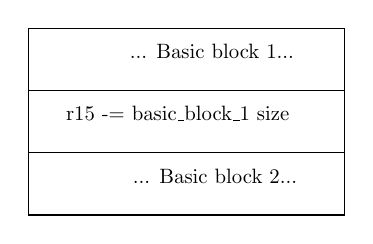
\begin{tikzpicture}[x=0.75pt,y=0.75pt,yscale=-1,xscale=1,scale=0.75, every node/.style={scale=0.75}]
%uncomment if require: \path (0,300); %set diagram left start at 0, and has height of 300

%Shape: Rectangle [id:dp67966345615795] 
\draw   (226,32) -- (429,32) -- (429,72) -- (226,72) -- cycle ;
%Shape: Rectangle [id:dp33759508561919027] 
\draw   (226,112) -- (429,112) -- (429,152) -- (226,152) -- cycle ;
%Shape: Rectangle [id:dp47015521373361546] 
\draw   (226,72) -- (429,72) -- (429,112) -- (226,112) -- cycle ;

% Text Node
\draw (290,41) node [anchor=north west][inner sep=0.75pt]   [align=left] {... Basic block 1...};
% Text Node
\draw (292,121) node [anchor=north west][inner sep=0.75pt]   [align=left] {... Basic block 2...};
% Text Node
\draw (249,81) node [anchor=north west][inner sep=0.75pt]   [align=left] {r15 -= basic\_block\_1 size};

\end{tikzpicture}
\end{tightcenter}
If it is not time then we should skip the rest of the tally code instructions and continue the original code. We do so by doing a conditional jump to a ``continue label''. \textbf{For our context switch mechanism to work, every continue label must have a unique id.}



\begin{tightcenter}
\tikzset{every picture/.style={line width=0.75pt}} %set default line width to 0.75pt        


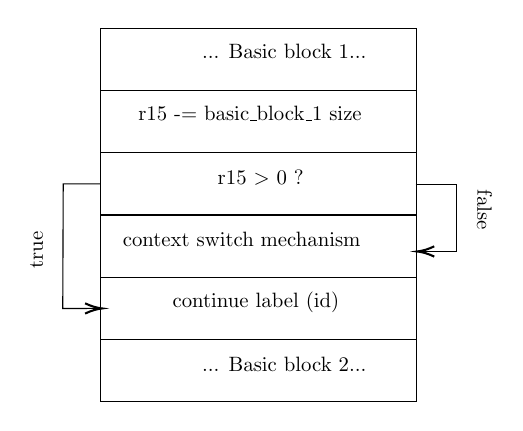
\begin{tikzpicture}[x=0.75pt,y=0.75pt,yscale=-1,xscale=1,scale=0.75, every node/.style={scale=0.75}]
%uncomment if require: \path (0,436); %set diagram left start at 0, and has height of 436

%Shape: Rectangle [id:dp2730471173363307] 
\draw   (223,35) -- (426,35) -- (426,75) -- (223,75) -- cycle ;
%Shape: Rectangle [id:dp7647299317107666] 
\draw   (223,115) -- (426,115) -- (426,155) -- (223,155) -- cycle ;
%Shape: Rectangle [id:dp2539580680672877] 
\draw   (223,155) -- (426,155) -- (426,195) -- (223,195) -- cycle ;
%Shape: Rectangle [id:dp26522572497418473] 
\draw   (223,75) -- (426,75) -- (426,115) -- (223,115) -- cycle ;
%Shape: Rectangle [id:dp6379141142291754] 
\draw   (223,195) -- (426,195) -- (426,235) -- (223,235) -- cycle ;
%Shape: Rectangle [id:dp9468927652009763] 
\draw   (223,235) -- (426,235) -- (426,275) -- (223,275) -- cycle ;
%Straight Lines [id:da5654882360859104] 
\draw    (223,135) -- (199,135) -- (198.7,215.03) -- (222,215) ;
\draw [shift={(224,215)}, rotate = 179.94] [color={rgb, 255:red, 0; green, 0; blue, 0 }  ][line width=0.75]    (10.93,-3.29) .. controls (6.95,-1.4) and (3.31,-0.3) .. (0,0) .. controls (3.31,0.3) and (6.95,1.4) .. (10.93,3.29)   ;
%Straight Lines [id:da9628834864645601] 
\draw    (425.41,135.41) -- (451.41,135.41) -- (451.41,178.41) -- (428.41,178.41) ;
\draw [shift={(426.41,178.41)}, rotate = 360] [color={rgb, 255:red, 0; green, 0; blue, 0 }  ][line width=0.75]    (10.93,-3.29) .. controls (6.95,-1.4) and (3.31,-0.3) .. (0,0) .. controls (3.31,0.3) and (6.95,1.4) .. (10.93,3.29)   ;

% Text Node
\draw (287,44) node [anchor=north west][inner sep=0.75pt]   [align=left] {... Basic block 1...};
% Text Node
\draw (287,245) node [anchor=north west][inner sep=0.75pt]   [align=left] {... Basic block 2...};
% Text Node
\draw (246,84) node [anchor=north west][inner sep=0.75pt]   [align=left] {r15 -= basic\_block\_1 size};
% Text Node
\draw (297,125) node [anchor=north west][inner sep=0.75pt]   [align=left] {r15 $>$ 0 ?};
% Text Node
\draw (268,203) node [anchor=north west][inner sep=0.75pt]   [align=left] {continue label (id)};
% Text Node
\draw (236,165) node [anchor=north west][inner sep=0.75pt]   [align=left] {context switch mechanism};
% Text Node
\draw (176.52,190.52) node [anchor=north west][inner sep=0.75pt]  [rotate=-269.92] [align=left] {true};
% Text Node
\draw (475.69,137.62) node [anchor=north west][inner sep=0.75pt]  [rotate=-90.58] [align=left] {false};


\end{tikzpicture}
\end{tightcenter}
If the tally variable is negative or zero, then it's time to do the context switch, and we call the switch function. We do so by way of a ``goto'' instruction to a specific point in the thread manager's code, with the \_minithread\_break label. This is similar to calling a function, but it preserves the stack and every register other than the instruction pointer (IP). 

This ``goto'' instruction can be done by pushing the \_minithread\_label onto to the stack and then executing a return instruction. A return instruction removes the top of the stack and puts that value on the instruction pointer. The context switching function of the thread manager, which contains the \_minithread\_break label, will be explained below.



\tikzset{every picture/.style={line width=0.75pt}} %set default line width to 0.75pt        
\begin{tightcenter}

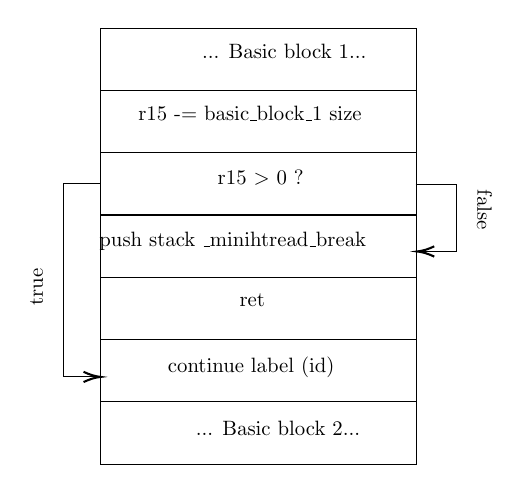
\begin{tikzpicture}[x=0.75pt,y=0.75pt,yscale=-1,xscale=1,scale=0.75, every node/.style={scale=0.75}]
%uncomment if require: \path (0,436); %set diagram left start at 0, and has height of 436

%Shape: Rectangle [id:dp2730471173363307] 
\draw   (223,35) -- (426,35) -- (426,75) -- (223,75) -- cycle ;
%Shape: Rectangle [id:dp7647299317107666] 
\draw   (223,115) -- (426,115) -- (426,155) -- (223,155) -- cycle ;
%Shape: Rectangle [id:dp2539580680672877] 
\draw   (223,155) -- (426,155) -- (426,195) -- (223,195) -- cycle ;
%Shape: Rectangle [id:dp26522572497418473] 
\draw   (223,75) -- (426,75) -- (426,115) -- (223,115) -- cycle ;
%Shape: Rectangle [id:dp6379141142291754] 
\draw   (223,195) -- (426,195) -- (426,235) -- (223,235) -- cycle ;
%Shape: Rectangle [id:dp9468927652009763] 
\draw   (223,235) -- (426,235) -- (426,275) -- (223,275) -- cycle ;
%Straight Lines [id:da5654882360859104] 
\draw    (223,135) -- (199,135) -- (199,259) -- (221,259) ;
\draw [shift={(223,259)}, rotate = 180] [color={rgb, 255:red, 0; green, 0; blue, 0 }  ][line width=0.75]    (10.93,-3.29) .. controls (6.95,-1.4) and (3.31,-0.3) .. (0,0) .. controls (3.31,0.3) and (6.95,1.4) .. (10.93,3.29)   ;
%Straight Lines [id:da9628834864645601] 
\draw    (425.41,135.41) -- (451.41,135.41) -- (451.41,178.41) -- (428.41,178.41) ;
\draw [shift={(426.41,178.41)}, rotate = 360] [color={rgb, 255:red, 0; green, 0; blue, 0 }  ][line width=0.75]    (10.93,-3.29) .. controls (6.95,-1.4) and (3.31,-0.3) .. (0,0) .. controls (3.31,0.3) and (6.95,1.4) .. (10.93,3.29)   ;
%Shape: Rectangle [id:dp8633088881890016] 
\draw   (223,275) -- (426,275) -- (426,315) -- (223,315) -- cycle ;

% Text Node
\draw (287,44) node [anchor=north west][inner sep=0.75pt]   [align=left] {... Basic block 1...};
% Text Node
\draw (283,286) node [anchor=north west][inner sep=0.75pt]   [align=left] {... Basic block 2...};
% Text Node
\draw (246,84) node [anchor=north west][inner sep=0.75pt]   [align=left] {r15 -= basic\_block\_1 size};
% Text Node
\draw (297,125) node [anchor=north west][inner sep=0.75pt]   [align=left] {r15 $>$ 0 ?};
% Text Node
\draw (265,245) node [anchor=north west][inner sep=0.75pt]   [align=left] {continue label (id)};
% Text Node
\draw (221,165) node [anchor=north west][inner sep=0.75pt]   [align=left] {push stack \_minihtread\_break};
% Text Node
\draw (176.52,214.52) node [anchor=north west][inner sep=0.75pt]  [rotate=-269.92] [align=left] {true};
% Text Node
\draw (475.69,137.62) node [anchor=north west][inner sep=0.75pt]  [rotate=-90.58] [align=left] {false};
% Text Node
\draw (311,204) node [anchor=north west][inner sep=0.75pt]   [align=left] {ret};

\end{tikzpicture}
\end{tightcenter}
In the above description of the context switch mechanism, we are still missing the address from were the context switch was activated. This is necessary so that we can switch back. This problem is then solved with the help of the continue label, since it gives us the exact point were we want to resume the execution of the minithread. Putting that label on the stack \textit{before} the \_minithread\_break label causes the continue label to sit at the top of the stack, once the return instruction is executed. The continue label is precisely the address of the instruction that we need to go to if we wish to continue the execution of the minithread.


\tikzset{every picture/.style={line width=0.75pt}} %set default line width to 0.75pt        

\begin{tightcenter}
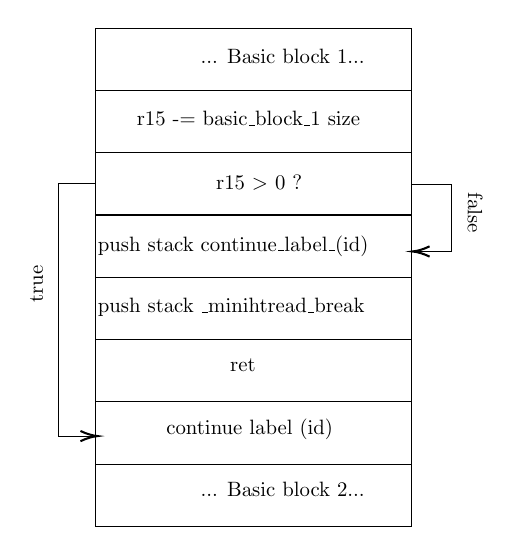
\begin{tikzpicture}[x=0.75pt,y=0.75pt,yscale=-1,xscale=1,scale=0.75, every node/.style={scale=0.75}]
%uncomment if require: \path (0,436); %set diagram left start at 0, and has height of 436

%Shape: Rectangle [id:dp2730471173363307] 
\draw   (223,35) -- (426,35) -- (426,75) -- (223,75) -- cycle ;
%Shape: Rectangle [id:dp7647299317107666] 
\draw   (223,115) -- (426,115) -- (426,155) -- (223,155) -- cycle ;
%Shape: Rectangle [id:dp2539580680672877] 
\draw   (223,155) -- (426,155) -- (426,195) -- (223,195) -- cycle ;
%Shape: Rectangle [id:dp26522572497418473] 
\draw   (223,75) -- (426,75) -- (426,115) -- (223,115) -- cycle ;
%Shape: Rectangle [id:dp6379141142291754] 
\draw   (223,195) -- (426,195) -- (426,235) -- (223,235) -- cycle ;
%Shape: Rectangle [id:dp9468927652009763] 
\draw   (223,235) -- (426,235) -- (426,275) -- (223,275) -- cycle ;
%Straight Lines [id:da5654882360859104] 
\draw    (223,135) -- (199,135) -- (199,297) -- (222,297) ;
\draw [shift={(224,297)}, rotate = 180] [color={rgb, 255:red, 0; green, 0; blue, 0 }  ][line width=0.75]    (10.93,-3.29) .. controls (6.95,-1.4) and (3.31,-0.3) .. (0,0) .. controls (3.31,0.3) and (6.95,1.4) .. (10.93,3.29)   ;
%Straight Lines [id:da9628834864645601] 
\draw    (425.41,135.41) -- (451.41,135.41) -- (451.41,178.41) -- (428.41,178.41) ;
\draw [shift={(426.41,178.41)}, rotate = 360] [color={rgb, 255:red, 0; green, 0; blue, 0 }  ][line width=0.75]    (10.93,-3.29) .. controls (6.95,-1.4) and (3.31,-0.3) .. (0,0) .. controls (3.31,0.3) and (6.95,1.4) .. (10.93,3.29)   ;
%Shape: Rectangle [id:dp7771689415503763] 
\draw   (223,315) -- (426,315) -- (426,355) -- (223,355) -- cycle ;
%Shape: Rectangle [id:dp8633088881890016] 
\draw   (223,275) -- (426,275) -- (426,315) -- (223,315) -- cycle ;

% Text Node
\draw (289,47) node [anchor=north west][inner sep=0.75pt]   [align=left] {... Basic block 1...};
% Text Node
\draw (289,325) node [anchor=north west][inner sep=0.75pt]   [align=left] {... Basic block 2...};
% Text Node
\draw (248,87) node [anchor=north west][inner sep=0.75pt]   [align=left] {r15 -= basic\_block\_1 size};
% Text Node
\draw (299,128) node [anchor=north west][inner sep=0.75pt]   [align=left] {r15 $>$ 0 ?};
% Text Node
\draw (267,285) node [anchor=north west][inner sep=0.75pt]   [align=left] {continue label (id)};
% Text Node
\draw (223,207) node [anchor=north west][inner sep=0.75pt]   [align=left] {push stack \_minihtread\_break};
% Text Node
\draw (179.52,212.51) node [anchor=north west][inner sep=0.75pt]  [rotate=-269.92] [align=left] {true};
% Text Node
\draw (472.67,139.59) node [anchor=north west][inner sep=0.75pt]  [rotate=-90.58] [align=left] {false};
% Text Node
\draw (308,246) node [anchor=north west][inner sep=0.75pt]   [align=left] {ret};
% Text Node
\draw (223,167) node [anchor=north west][inner sep=0.75pt]   [align=left] {push stack continue\_label\_(id)};
\end{tikzpicture}
\end{tightcenter}


\subsection{The context-switching function: switch out}\label{switch out function}

\_minithread\_break is the label that represents the point in the thread manager's context switch function, where the execution context of the minithread is saved, and the execution context of the thread manager is restored. Please look at Section \ref{context macros}, where we list the C code for the context-switch function. Here we are insterested in the second half of this C code, beginning with the \_minithread\_break label, which is goto'ed whenever a minithread pauses execution.

At the \_minithread\_break point (line \ref{minithread break label}), the context-switch function starts by calling the macro PUSH\_REGISTERS, which pushes all of the minithread's registers to the top of the minithread's stack. This needs to be the first step, since any code written in C will use the various available registers, and so any such code would alter the execution context of the minithread. The minithread's current stack pointer is saved immediately after (line \ref{save sp}), using extended assembly, to a thread-local variable \_thread\_sp, which will eventually be stored in the minithread's data structure. We store the stack pointer on a variable instead of also putting it on the minithread stack to easily access it when checking the minihtread return state,     (see Section \ref{exit state}).

Now that the environment of the minithread is stored we can change the stack pointer to point to the stack of the thread manager (line \ref{put sp}), and restore the thread manager's context with the POP\_REGISTERS (\ref{context macros}) macro.

Why didn't we save the IP that was on the stack? When restoring the context of the minithread we need to pop all registers from the stack to their correct place and this will leave us with the correct continue label address on top. Then we may resume the minithread simply by calling a return instruction, and this will jump to the correct place in the instrumented code.

\subsection{The context-switching function: switch in}

By giving control to the instrumented function and expecting control to come back we need to save the environment of the thread manager, which will later be restored when the minithread pauses execution.  

We can save our environment by using a similar procedure as in the context switch-in, by only inverting which stack pointer and registers are saved and restored. Also, we need to consider the case when the minithread is starting execution for the first time, since then its stack will not have any prior saved state registers to pop. Naturally, the thread manager's registers need to be saved on the thread manager's stack, and the minithread registers will be in the minithread's stack.

If we are executing the minithread for the first time, we simply call the appropriate function pointer (line \ref{call func}), which is stored in the minithread. We may do this simply using C code, as it even allows us to pass arguments to this initial call, while remaining compatible with calling conventions, \textit{etc}. 

If, instead, we are resuming the execution of the minithread we first need to use the POP\_REGISTER (\ref{context macros}) macro to restore its environment (line \ref{pop regs}). As per the context-switch protocol, this will leave the appropriate continue label on top of the stack, and thus, to resume the minithread execution, we only need to execute an assembly return instruction (line \ref{ret instr}).

By placing the context switch-out code (\_minithread\_break label) after the context switch-in code, we also resolve the case where the instrumented function exits by its own means like by executing a return type instruction.

In the current implementation of our switch-in function we use a \_thread\_local variable to pass values from before to after switching stacks. We need to do this for a minithread reference after switching stacks is needed. This can be done because at least on \textit{Linux} and using \textit{Gcc} as \_thread\_local variables are not stored on the current context stack. As an alternative for when this assumptions are not true we also provide a different implementation where instead of \_thread\_local variables register variables are used to keep the reference to the minithread.

\subsection{Exit state} \label{exit state}

By looking at the minithread stack state we can see if the control flow arrived at \_minithread\_break because of a context switch-out (i.e. a forced or voluntary yield, or an interrupt) or by a return instruction (meaning, the minithread function itself returned).

If the function itself has returned, this means that it consumed the bottom of the minithread's stack by calling {\tt ret} on the label placed that was placed there when the manager called the function for the first time (line \ref{call func} of the code \ref{context code}). So at that point the minithread's stack is empty. Then, the PUSH\_REGISTERS instruction (line \ref{push regs}) will add the registers on top of the minithread's stack. This takes up 30 words on the stack. So, if the function returned by itself, the stack will have size exactly 30.  If, instead, the minithread was paused (by a yield or interrupt), then after the switch-out the minithread will have a stack strictly larger than 30 (because it contains at least 30 registers plus the return address for the function call).

So if the stack has size 30, the exit state is MINITHREAD\_RETURNED. Otherwise, it is one of the paused states: MINITHREAD\_FORCED\_YIELD,\\ MINITHREAD\_VOLUNTARY\_YIELD, or MINITHREAD\_INTERRUPT. If the thread did a voluntary yield or an interrupt, this operation already changed the minithread's state accordingly. If, however, the minithread did a forced yield, then the state of the minithread after the context switch-out is MINITHREAD\_RUNNING, and it is then changed to MINITHREAD\_FORCED\_YIELD.
 

\subsection{Obtaining the tally}\label{instrumentation estimate}

As mention above in Chapter \ref{overview} we take advantage of GCC GIMPLE code structure of basic blocks to minimize the number of instructions in the context switching mechanism, while at the same time ensuring we count every single instruction that is executed.

We now know how the context switch-in and switch-out are implemented. But the following important detail was left hidden under the rug: how does one estimate the number of instructions in each basic\_block?

The issue is that, at the GCC compiler GIMPLE stage, each ``instruction'' is not a basic assembly instruction, but rather it is a GIMPLE instruction. These GIMPLE instructions are not exactly assembly instructions: they are potentially more complicated. e.i. A complex variable assignment (var x = 2 * f(3,4) + a ) is only one GIMPLE instruction but has many sub operations were each requires multiple assembly instructions .  

As a result, a single GIMPLE instruction can correspond to several assembly instructions in the final assembly code. So we have no hope of learning the exact number of assembly instructions which will appear in a given basic\_block at this stage of compilation. The best that we can get is a rough estimate.

By iterating through every basic block and analysing not only the number of instruction contained in each block but also the number of operators each one has we can better estimate the CPU cycles cost of every block.


%\subsection{Instrumentation locations} \label{instumentation location}
%So now we have a context switch mechanism so where do we insert it? And how do we decrease our tally?

%The first instinct is to check every instruction, so we would execute an instruction subtract one from the tally and them run our switch mechanism described above.

%With this method we can already see the problem that we would spend more cpu time checking is its time to run a context switch then running the code itself. 

%Can we instead of doing it every instruction do it every n instructions? No, not with a constant size, imagine that in a block of n instructions we have a jump in the middle to outside of the block, basically the instructions until the jump would not be counted. 

%The actual solution is already built in in one of the compilation phases. Gcc runs two three-address representations of the code, one of them being GIMPLE, in this phase the code is separated in basic\_blocks, \textquotesingle A basic block is a straight-line sequence of code with only one entry point and only one exit\textquotesingle.

%Our plugin is called in the GIMPLE stage of compilation, and for every basic block it counts the instructions for the block and before the exit point it subtracts from the tally the number of instructions and runs the context switch mechanism this way we guarantee that we count every instruction, and we are minimizing the amount of extra instructions added.

\subsection{Context switch-out branch predictor optimization} \label{bpo}
Modern CPUs use a technique of branch prediction to try to speed code execution \cite{bpo} by trying to guess which path of an if-else or conditional jump instruction the code is going to follow. 

The \cite{Intel} manual references, in its Section 3.4.1.2, what branch is predicted when encountering a conditional jump:
\begin{itemize}
    \item Predict forward conditional branches to be NOT taken.
    \item Predict backward conditional branches to be taken.
\end{itemize}


Using the mechanism described above, and with the knowledge of the preferred branch of the branch predictor, we find that the branch predictor, if following the above rule of not taking forward branches, will always predict in favor of the context-switching code, instead of the rest of the minithread's code.

We can change this as follows. We first split the mechanism into two parts: (1) the decrement of the tally variable and the conditional jump, and (2) the switch-out code. We keep part 1 in the same place as before. And we place all the different part 2s (the switch-out code part, there is one such part for every basic\_block) at the end. (Because of the way the compiler plugin works, all the switch-out codes corresponding to each function are placed together at the end of the function.) This is illustrated in the figure below.

Then, if the tally is zero or negative, we jump to the corresponding switch-out code (part 2). This is now a forward jump, hence the branch predictor will predict against the jump, and instead predict in favor of the minithread's own code.

Using this knowledge we can try to optimize our context switch mechanism so the branch predictor always takes the path to execute more code instead of evaluating the mechanism. This is helpful as we predict that more times than none we are continuing execution of the minithread's code, instead of executing a switch. This causes branch prediction and speculative execution to favor the minithread's own code.


\begin{tightcenter}

\tikzset{every picture/.style={line width=0.75pt}} %set default line width to 0.75pt        

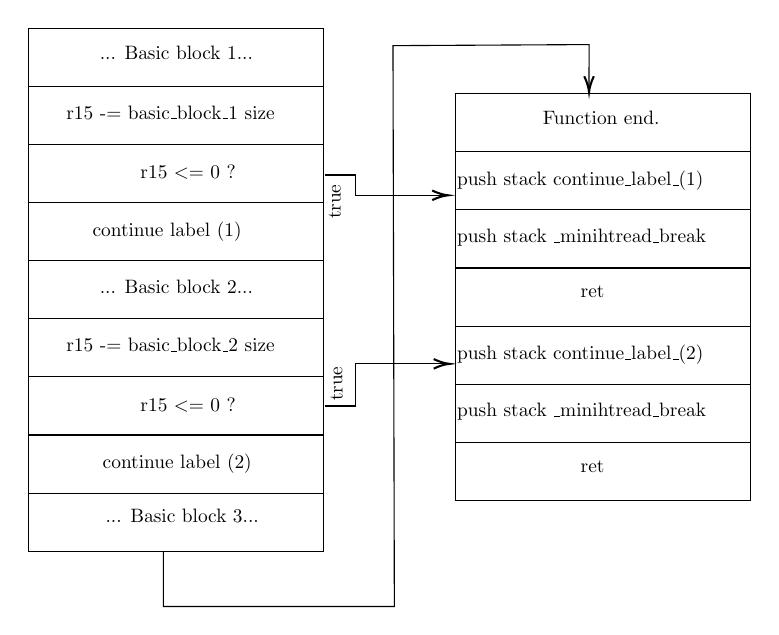
\begin{tikzpicture}[x=0.75pt,y=0.75pt,yscale=-1,xscale=1,scale=0.7, every node/.style={scale=0.7}]
%uncomment if require: \path (0,914); %set diagram left start at 0, and has height of 914

%Shape: Rectangle [id:dp2730471173363307] 
\draw   (94,39) -- (297,39) -- (297,79) -- (94,79) -- cycle ;
%Shape: Rectangle [id:dp7647299317107666] 
\draw   (94,119) -- (297,119) -- (297,159) -- (94,159) -- cycle ;
%Shape: Rectangle [id:dp2539580680672877] 
\draw   (388,124) -- (591,124) -- (591,164) -- (388,164) -- cycle ;
%Shape: Rectangle [id:dp26522572497418473] 
\draw   (94,79) -- (297,79) -- (297,119) -- (94,119) -- cycle ;
%Shape: Rectangle [id:dp6379141142291754] 
\draw   (388,164) -- (591,164) -- (591,204) -- (388,204) -- cycle ;
%Shape: Rectangle [id:dp9468927652009763] 
\draw   (388,204) -- (591,204) -- (591,244) -- (388,244) -- cycle ;
%Straight Lines [id:da5654882360859104] 
\draw    (298,140) -- (319,140) -- (319,154) -- (381,154) ;
\draw [shift={(383,154)}, rotate = 180] [color={rgb, 255:red, 0; green, 0; blue, 0 }  ][line width=0.75]    (10.93,-3.29) .. controls (6.95,-1.4) and (3.31,-0.3) .. (0,0) .. controls (3.31,0.3) and (6.95,1.4) .. (10.93,3.29)   ;
%Straight Lines [id:da9628834864645601] 
\draw    (187,399) -- (187,437) -- (346,437) -- (345.06,50.99) -- (480.01,50.25) -- (480,81) ;
\draw [shift={(480,83)}, rotate = 270.01] [color={rgb, 255:red, 0; green, 0; blue, 0 }  ][line width=0.75]    (10.93,-3.29) .. controls (6.95,-1.4) and (3.31,-0.3) .. (0,0) .. controls (3.31,0.3) and (6.95,1.4) .. (10.93,3.29)   ;
%Shape: Rectangle [id:dp7771689415503763] 
\draw   (94,199) -- (297,199) -- (297,239) -- (94,239) -- cycle ;
%Shape: Rectangle [id:dp17936857993525634] 
\draw   (94,279) -- (297,279) -- (297,319) -- (94,319) -- cycle ;
%Shape: Rectangle [id:dp46920471530816465] 
\draw   (94,239) -- (297,239) -- (297,279) -- (94,279) -- cycle ;
%Shape: Rectangle [id:dp11744847492899946] 
\draw   (94,319) -- (297,319) -- (297,359) -- (94,359) -- cycle ;
%Shape: Rectangle [id:dp6198967254102352] 
\draw   (94,159) -- (297,159) -- (297,199) -- (94,199) -- cycle ;
%Shape: Rectangle [id:dp9175047436043668] 
\draw   (94,359) -- (297,359) -- (297,399) -- (94,399) -- cycle ;
%Shape: Rectangle [id:dp4090865488505543] 
\draw   (388,84) -- (591,84) -- (591,124) -- (388,124) -- cycle ;
%Shape: Rectangle [id:dp46132806280731364] 
\draw   (388,244) -- (591,244) -- (591,284) -- (388,284) -- cycle ;
%Shape: Rectangle [id:dp6054839709956552] 
\draw   (388,284) -- (591,284) -- (591,324) -- (388,324) -- cycle ;
%Shape: Rectangle [id:dp8829802167865602] 
\draw   (388,324) -- (591,324) -- (591,364) -- (388,364) -- cycle ;
%Straight Lines [id:da6407126083495657] 
\draw    (298,299) -- (319,299) -- (319,270) -- (382,270) ;
\draw [shift={(384,270)}, rotate = 180] [color={rgb, 255:red, 0; green, 0; blue, 0 }  ][line width=0.75]    (10.93,-3.29) .. controls (6.95,-1.4) and (3.31,-0.3) .. (0,0) .. controls (3.31,0.3) and (6.95,1.4) .. (10.93,3.29)   ;

% Text Node
\draw (142,50) node [anchor=north west][inner sep=0.75pt]   [align=left] {... Basic block 1...};
% Text Node
\draw (142,211) node [anchor=north west][inner sep=0.75pt]   [align=left] {... Basic block 2...};
% Text Node
\draw (119,91) node [anchor=north west][inner sep=0.75pt]   [align=left] {r15 -= basic\_block\_1 size};
% Text Node
\draw (170,132) node [anchor=north west][inner sep=0.75pt]   [align=left] {r15 $<=$ 0 ?};
% Text Node
\draw (137,171) node [anchor=north west][inner sep=0.75pt]   [align=left] {continue label (1)};
% Text Node
\draw (388,176) node [anchor=north west][inner sep=0.75pt]   [align=left] {push stack \_minihtread\_break};
% Text Node
\draw (299.52,171.51) node [anchor=north west][inner sep=0.75pt]  [rotate=-269.92] [align=left] {true};
% Text Node
\draw (300.97,296.96) node [anchor=north west][inner sep=0.75pt]  [rotate=-269.22] [align=left] {true};
% Text Node
\draw (473,215) node [anchor=north west][inner sep=0.75pt]   [align=left] {ret};
% Text Node
\draw (388,136) node [anchor=north west][inner sep=0.75pt]   [align=left] {push stack continue\_label\_(1)};
% Text Node
\draw (146,369) node [anchor=north west][inner sep=0.75pt]   [align=left] {... Basic block 3...};
% Text Node
\draw (119,251) node [anchor=north west][inner sep=0.75pt]   [align=left] {r15 -= basic\_block\_2 size};
% Text Node
\draw (170,292) node [anchor=north west][inner sep=0.75pt]   [align=left] {r15 $<=$ 0 ?};
% Text Node
\draw (144,331) node [anchor=north west][inner sep=0.75pt]   [align=left] {continue label (2)};
% Text Node
\draw (447,95) node [anchor=north west][inner sep=0.75pt]   [align=left] {Function end.};
% Text Node
\draw (388,296) node [anchor=north west][inner sep=0.75pt]   [align=left] {push stack \_minihtread\_break};
% Text Node
\draw (473,335) node [anchor=north west][inner sep=0.75pt]   [align=left] {ret};
% Text Node
\draw (388,256) node [anchor=north west][inner sep=0.75pt]   [align=left] {push stack continue\_label\_(2)};


\end{tikzpicture}
\end{tightcenter}

\section{Modules} \label{modules}
Ideally, we would now do an instrumented compilation of the entire C standard. However, this would be a massive effort, and is beyond the scope of this project. More generally, the program using the minithread library might wish to provide its own functionality to the minithreads it runs. So we implemented a module system, which is designed to give minithreads access to a controlled and limited set of shared libraries (which may in turn be instrumented).

One of the first justifications to implement modules was to allow dynamic memory allocation inside the minithreads' code. If we use the normal system calls of malloc and free this memory is not counted for the total amount of memory used by each minithread. So we decided to implement a heap module where it uses some of the the stack space of the minithread for dynamic memory allocation. We adapted a opensource project called SHMALL \cite{SHMALL}.

The only other module we implemented was a graph module that allowed us to share a graph with all minithreads with a simple API.


\iffalse

%This module uses a structure as the entry point for the heap.
To stay with the philosophy that we should keep all memory related to the minithread in its stack we needed a way of reserving part of the minithreads stack memory of the module to use as its heap.
To be able to do this, when initializing a minithread our thread manager checks if each of the modules provided to that minithread has an init function (provided in the wrapper structured used to signal that the minithread should use that module, \ref{init minithread}) and executes it.

This lead us to separate each module into two parts. Clean code and instrumented code.

\iffalse
\subsection{Module structure}
When a module is initialized in a minithread a structure containing its information is allocated (the size needs to be provided in the module arguments structure). Inside the module structure should be declared a $gcctally\_module\_wrapper$ \textbf{as its first item}, this structure contains the module hash name, init function pointer, memory used on the minithreads stack. It is important that 
\fi

\subsection{Clean code}
Clean code is code that was not compiled with the plugin. 
In the clean code file of a module should contain every function used to initialize the module our interact with it outside of the minithreads instrumented function scope.

If the module requires any kind of initialization then a init function should be implemented here.
This init function should allocate the space needed by the module on the minithread stack and setup all the data needed for the module to function on the minithread.

A cleanup function can also be provided in the module wrapper for the thread manager to free memory allocated during initialization. At the moment when this report is being written the thread manager does not execute the cleanup function at any point but the infrastructure is there for future development.  

\subsection{Instrumented code}
In the instrumented code file should be all the functions provided by the module to be used during the minithreads execution. This file will be instrumented so all the cycles used by this functions can be counted for the cycles done by the minithread. 

If a module uses some kind of structure to keep its data and this structure is needed to execute some of its provided API a \textit{find} function is provided from the thread manager to locate the module structure in the minithread memory.  

This function is needed because the minithread should not be able to break its scope and have a reference to it self or to the structure defining it. 

\subsubsection{Finding module structure}
During the minithreads initialization its modules are initialized and a wrapper structure is created to store their beginning point on minithread's memory along with other information, this wrappers are sorted by their module's name hash on an array in the minithreads structure.

By sorting all the modules wrappers on initialization we are able to find the module needed only knowing its name, hashing with the included hash macro and doing a binary search on the array of the minithread pointer by threadInUse \ref{thread in use}


\fi
% -----------------------------------------------------------------------------
% End inlined source: ch3.tex
% -----------------------------------------------------------------------------
\clearpage
\clearpage
% -----------------------------------------------------------------------------
% Begin inlined source: ch4.tex
% -----------------------------------------------------------------------------
\chapter{Performance}

After the library was built, we needed to characterize its performance against all variables in the system.

These are some definitions that are used all during the analysis:

\textbf{ Metacycle } $\rightarrow$ calling minithread\_run\_cycles on every minithread in the program once

\textbf {Number\_of\_total\_cycles / Work } $\rightarrow$ amount of cycles ran during the program execution from all minithreads.

\textbf{ Number\_of\_cycles } $\rightarrow$ cycles ran by a minihtread during a call from minihtread\_run\_cycles.

\section{System Setup}
All benchmarks were performed on a Intel Xeon x5650 2.66ghz and 12MB of cache, running Ubuntu 20.04.4 LTS x86\_64 with 16gb of ram.

Every minithread was created with 1$<<$10 (1024) bytes of total memory and ran \qq{./code/random\_walk.c} on a 1000 node graph (graph.txt) so it would stay in cache the whole time.

Every data point was generated with a median of 100 samples, the data points as well as the scripts used to gather the data will be present on the GitHub page of this library (https://github.com/ILBSPT/Tally).

\subsection{Random Walk}
Random walk was the algorithm chosen to test the performance of our library. 

It's a simple infinite loop that starts on a node of the graph and every iteration chooses a random neighbor to that node to jump to. On the next iteration it will choose a neighbor from that new node to jump to and so on.   

\section{Code size increase}
Our plugin on average using small functions increased the binary file size of the functions by 100 to 200\%.

\section{Multiple file performance hit}
Our library relies on dlopen and dynamic libraries of instrumented code, so we predicted that this was where we might encounter the first bottleneck in the system, as the number of files increases there might be cache misses on code fecth when switching contexts.
%\todo[inline]{Our reasoning was: if we have multiple minithreads all running different code, then switching context from one minithread to another would lead to a lot of cache misses during code fetch.} 
We tested if there was a difference between multiple minithreads using the same library file versus each minithread using its own libary file (with the same function code).


\subsection{Setup}
We started with a constant number of minithreads (1e4), doing a constant amount of work, 100 cycles per minithreads for 1000 metacycles, then for each run we varied the number of different files opened and used, but always running the same function.

If dlopen is called on the same file twice, it is going to return the same pointer, so we cannot have two copies of the same library file open. Hence, for this experiment to work we needed to compile the file to a shared library and then create 10000 copies of it with different filenames.

We needed to stop the data collection at 10k copies as (our version of) dlopen gives segfault when trying to open more than circa 13k files.

\begin{figure}[hbt]
    \centering
    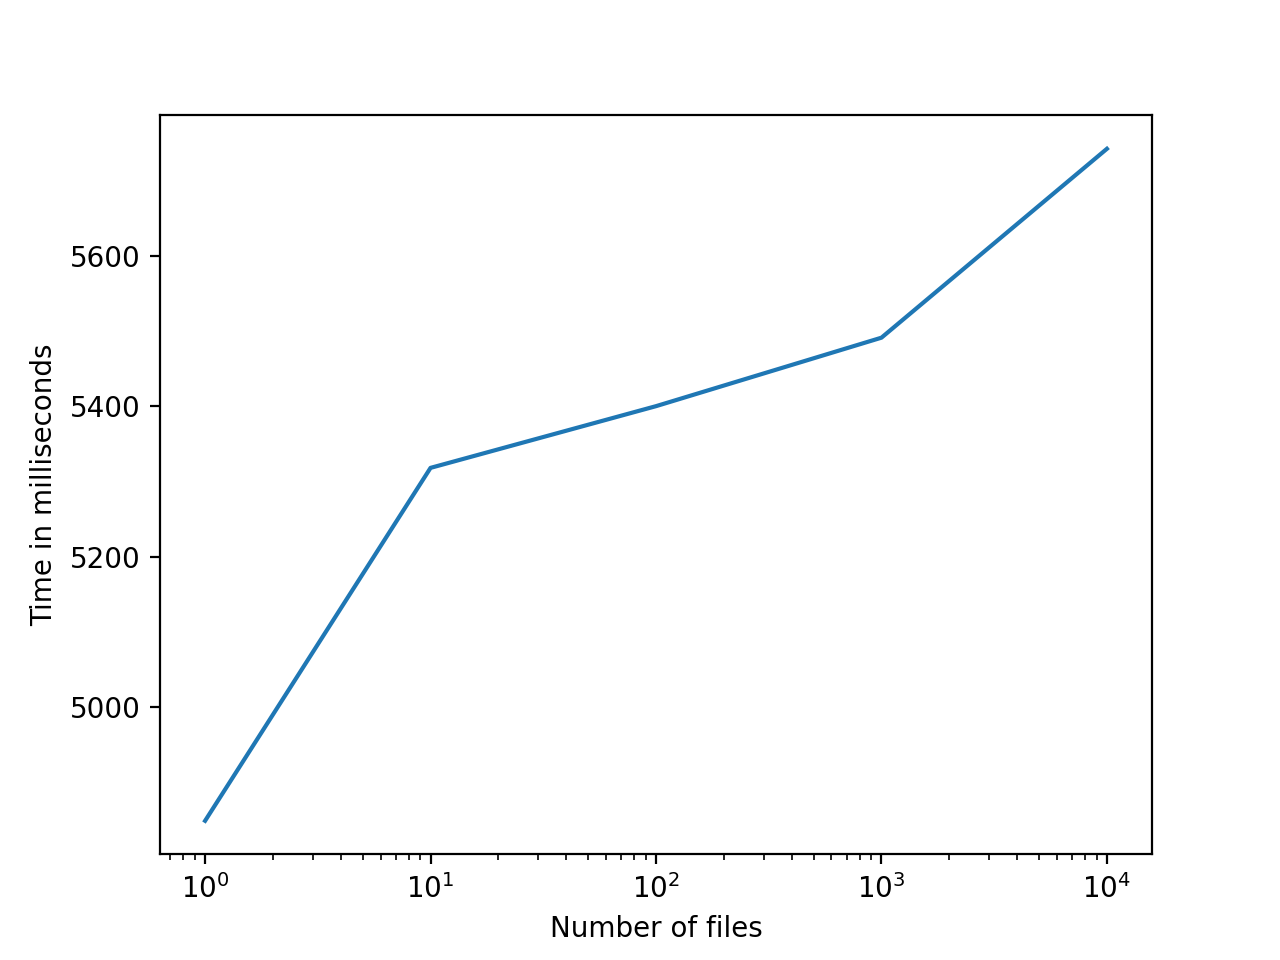
\includegraphics[width =0.7\textwidth]{images/teste3_cache_files.png}
    \caption{Performance hit from using different amount of files to accomplish 1e9 work from different minithreads configurations}
    \label{cache_files}
\end{figure}

\subsection{Findings}
We found just an 18\% increase in time taken when using 4 orders of magnitude more files,  figure \ref{cache_files}. Because of this finding all the data presented bellow will be gathered using the same file for every minithread as we fell that the 18\% increase is not enough to justify the added complexity of testing with multiple files.

\section{Multiple minithreads performance hit} \label{multi thread pref hit}
The next bottleneck that we needed to investigate was the penalty of using multiple minithreads as was our hypothesis that as the number of threads increases, we start to take cache miss penalties as we are unable to keep every minithread stack in cache.

We also tested if shuffling the order of execution of the minithread would have any kind of performance impact. This is to test if malloc allocates memory in a way beneficial to sequential reading.


\subsection{Setup}
To test this we ran 4 different setups with different amounts of total work: 1e7, \ldots, 1e10. Each minithread did 100 cycles per metacycle and because our only intention was to study the impact of the cache misses we used the formula:
\begin{equation}
    \text{number-of-metacycles} = \frac{\text{work}}{\text{number-of-minithreads} \times \text{number-of-cycles}}
\end{equation}
 to calculate the number of metacycles we needed to run and \textbf{keep the total number of context switches constant}, this way the only variance is the number of minithreads used. 
 
 \begin{figure}[hbt]
     \centering
     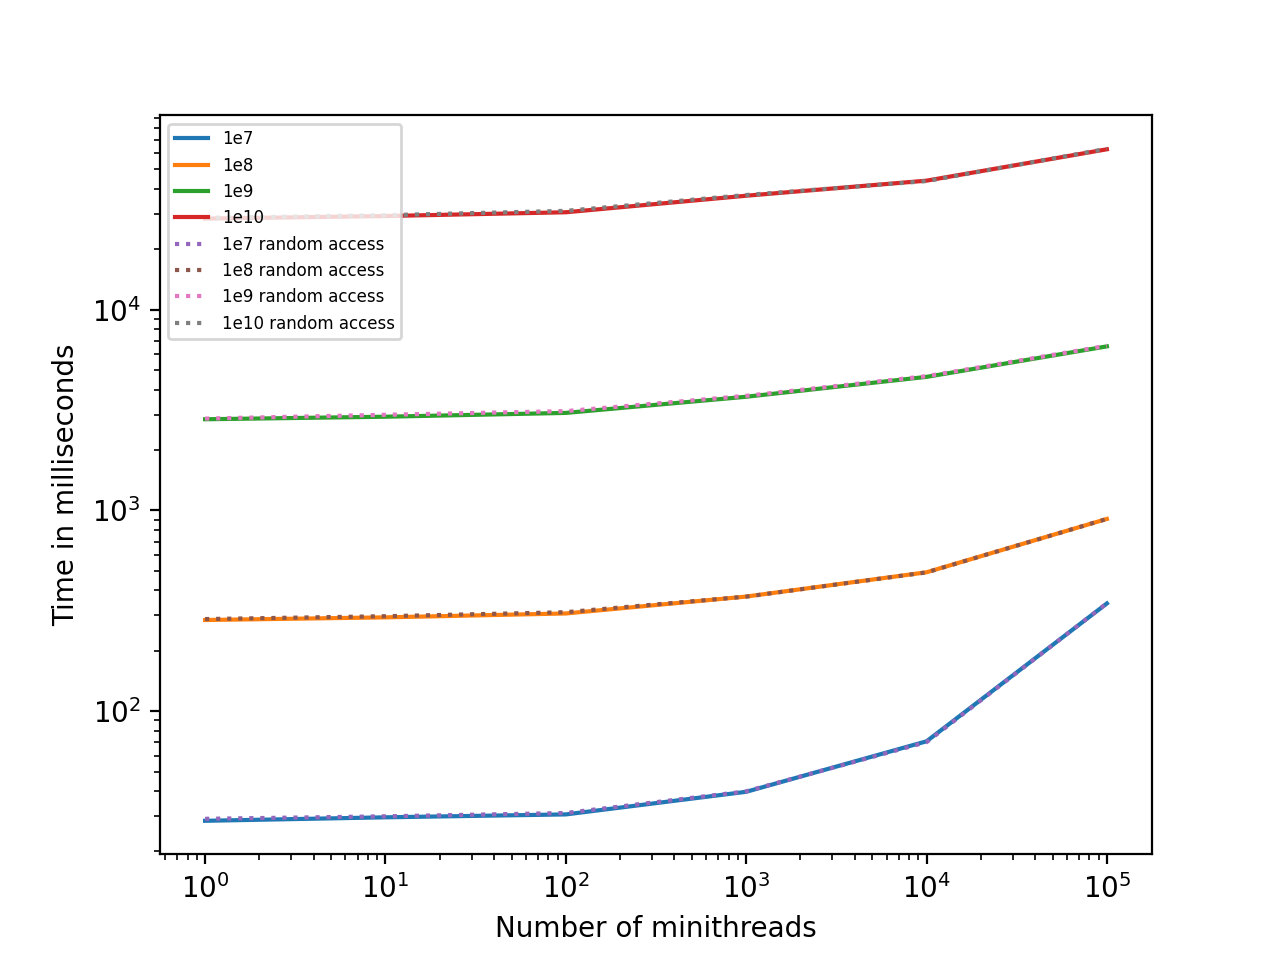
\includegraphics[width =0.85\textwidth]{images/teste2_diff_work.png}
     \caption{Performance hit from using multiple minithreads to perform some amount of work with the number of context switches being constant and 100 cycles per execution, log log scale}
     \label{cache_threads}
 \end{figure}
 
  \begin{figure}[hbt]
     \centering
     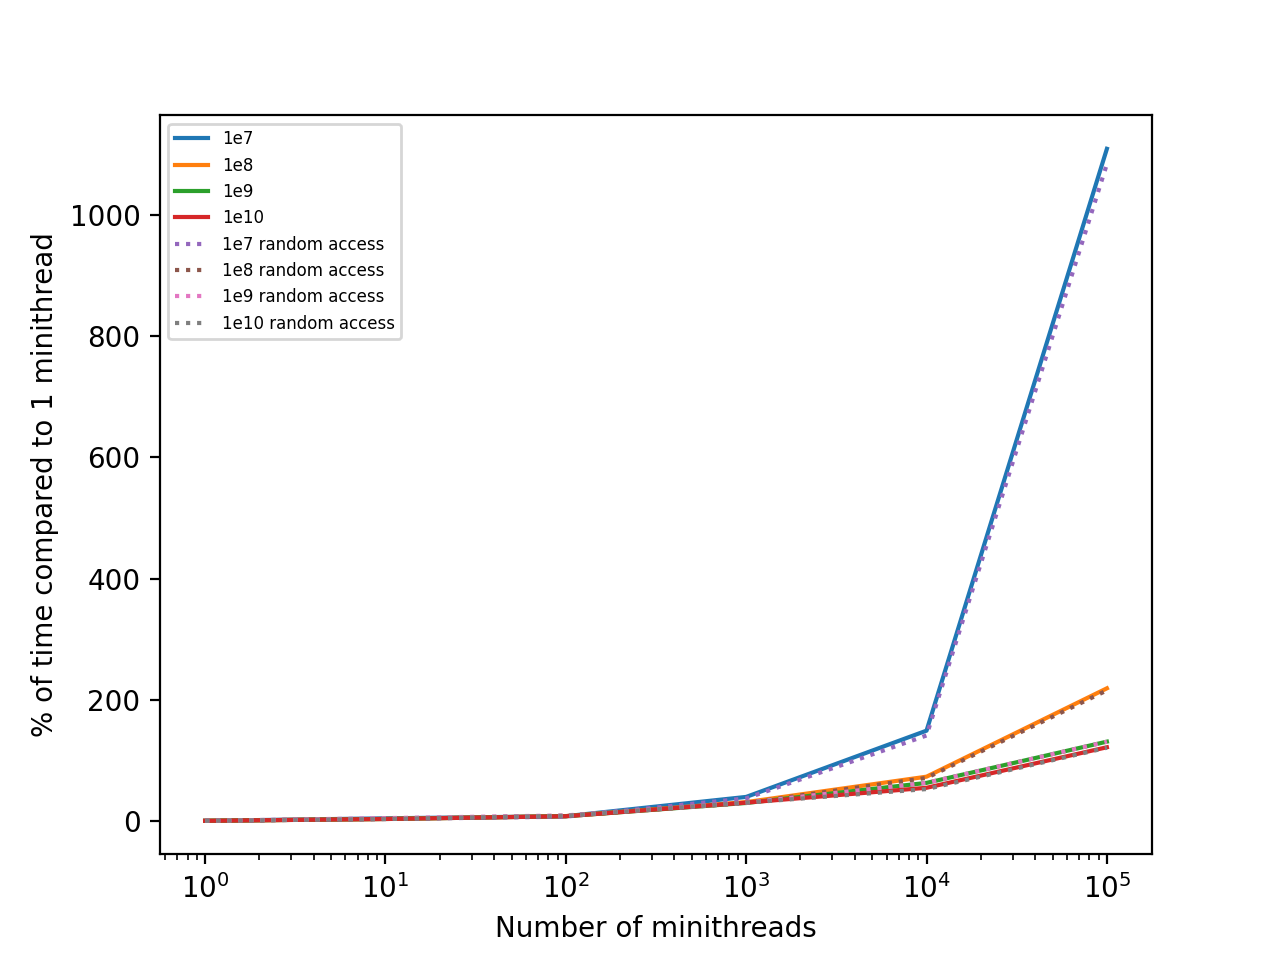
\includegraphics[width =0.85\textwidth]{images/teste2_diff_work_per.png}
     \caption{Percentage of time compared from using multiple minithreads to 1 minithread  when performing some amount of work with the number of context switches being constant and 100 cycles per execution}
     \label{cache_threads_per}
 \end{figure}
 
 \subsection{Findings}
 We can see (figures \ref{cache_threads}, \ref{cache_threads_per}) than the amount of time taken is proportional to the amount of work to do with 1 minithread, we can also see that when using multiple minithreads there is a greater performance hit went doing less work, running the minithreads on a shuffled order does not yield different results this leads us to believe that the order from witch the minithreads are initiated does not impacted their performance .
 
 \section{Branch prediction optimization}
 During the phase of development, we implemented a different order for the instructions that instrument the code so we could try to work with the branch predictor and sway the prediction to the branch that we thought has the right one most of the time. The whole description and theory behind the implementation is described in section \ref{bpo}.
 
 \subsection{Setup}
 To test if it works, we ran head-to-head comparisons of the same number of threads doing work ($2^{30}$ cycles) on a varying amount to metacycles, by varying the number of metacycles we are controlling the number of context switches done giving us the performance hit of the context switches in both instrumentation\textquotesingle s. The number of cycles ran by each minithread per metacyles was given by this formula:
 \begin{equation}
 \text{number-of-cycles} = \frac{\text{work}}{\text{number-of-minithreads} \times \text{number-of-metacycles}}
 \end{equation}
 
 \begin{figure}[hbt]
     \centering
     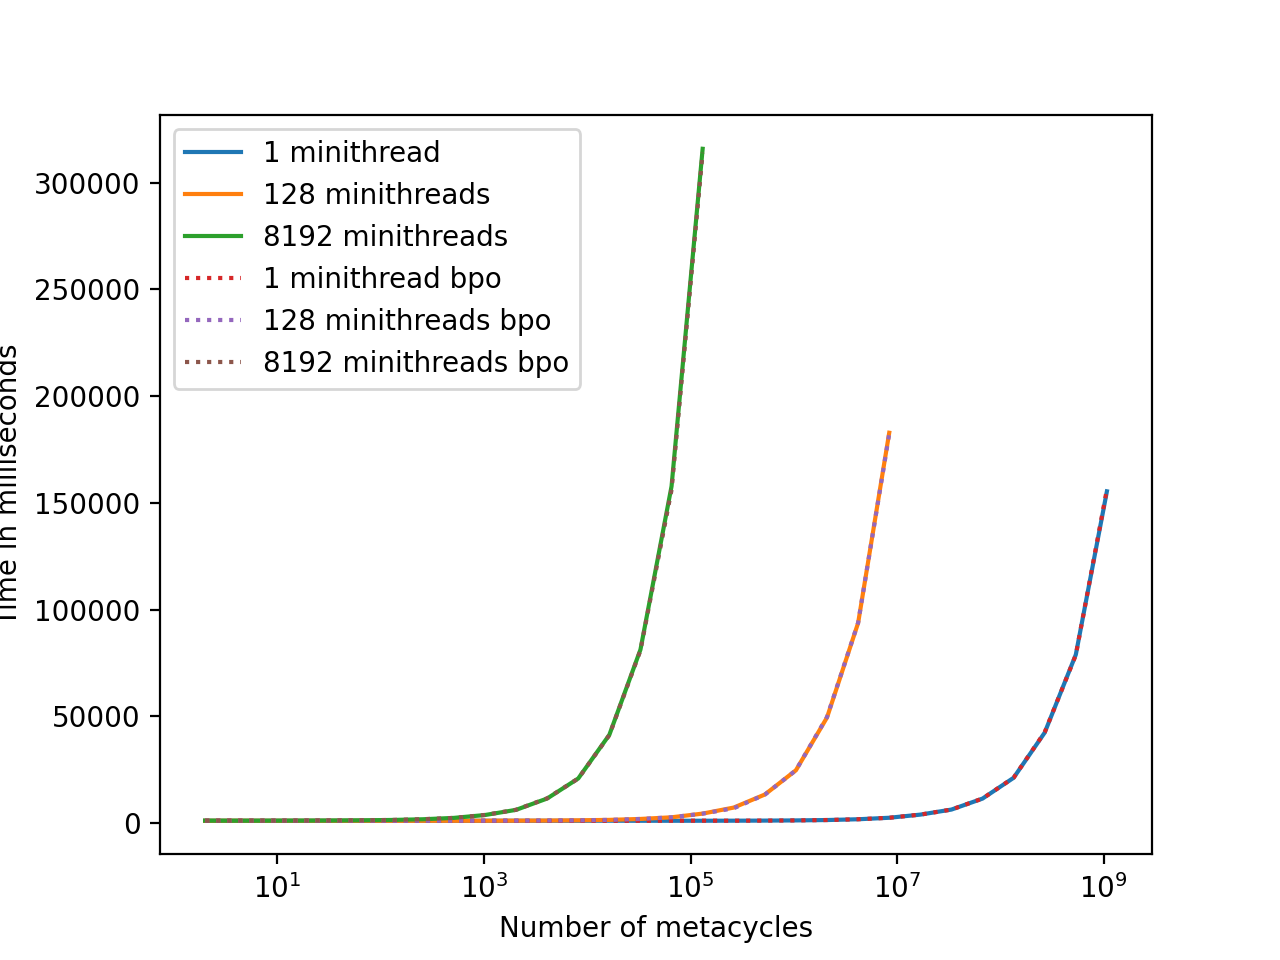
\includegraphics[width =0.7\textwidth]{images/teste4_context_switch_bpo_bin.png}
     \caption{Performance hit from using multiple metacycles to perform a constant amount of work($ 2^{30} $) for 1, 128 and 8192 minithreads and difference between using a normal context switch and a branch predictor optimized context switch(bpo)}
     \label{context_switch_bpo}
 \end{figure}
 
 \subsection{Findings}
 This (figure \ref{context_switch_bpo}) shows that a multi-billion-dollar company can outsmart a third-year project. There is no significant gain or loss in performance when trying to optimize for the branch predictor: it does equally well with both strategies we used.
 
 \textbf{Attention:} the overall performance for both setups is wrong and will be discussed why bellow, but for a head to head comparison it is still valid. 
 
\section{Calculating the cost of a context switch}
Calculating the cost of a context switch is important to know the practical lower limit of cycles that a minithread can run without spending more time during the switch that actually runing the minithread.

But before calculating this number we need to do some corrections on our context switch graph \ref{context_switch_bpo}.

\subsection{Overwork} \label{overwork}
 The results when running high numbers of metacycles intrigued us because of a sudden loss in performance. 
 Upon closer inspection we suspected that our minithreads were doing overwork (more work than the total work they were supposed to do) when the number of cycles per metacyle was closing on 0. This can happen because TALLY does not have enough granularity to only do a very small number of cycles per metacycle, because as it only checks the tally after each basic\_block \ref{instrumentation estimate}.
 
 We can expect an overwork of: $Cycles\_to\_run \: \% \: average\_basic\_block\_cost$ every time the run the minithread.
 
 So if we do a large amount of metacycles with only a few cycles each, we will end up with a negative tally on most metacycles, and so the minithread will do more work than what what it was supposed to do. 
 
 We can check how much extra work is being done by examining the tally of the minithread after each execution: if the tally is negative, then the minithread did more work than it should have done. If we add the absolute value of all these negative numbers, we end up with an estimate of how much overwork the minithread did.
 
\begin{figure}[hbt]
    \centering
    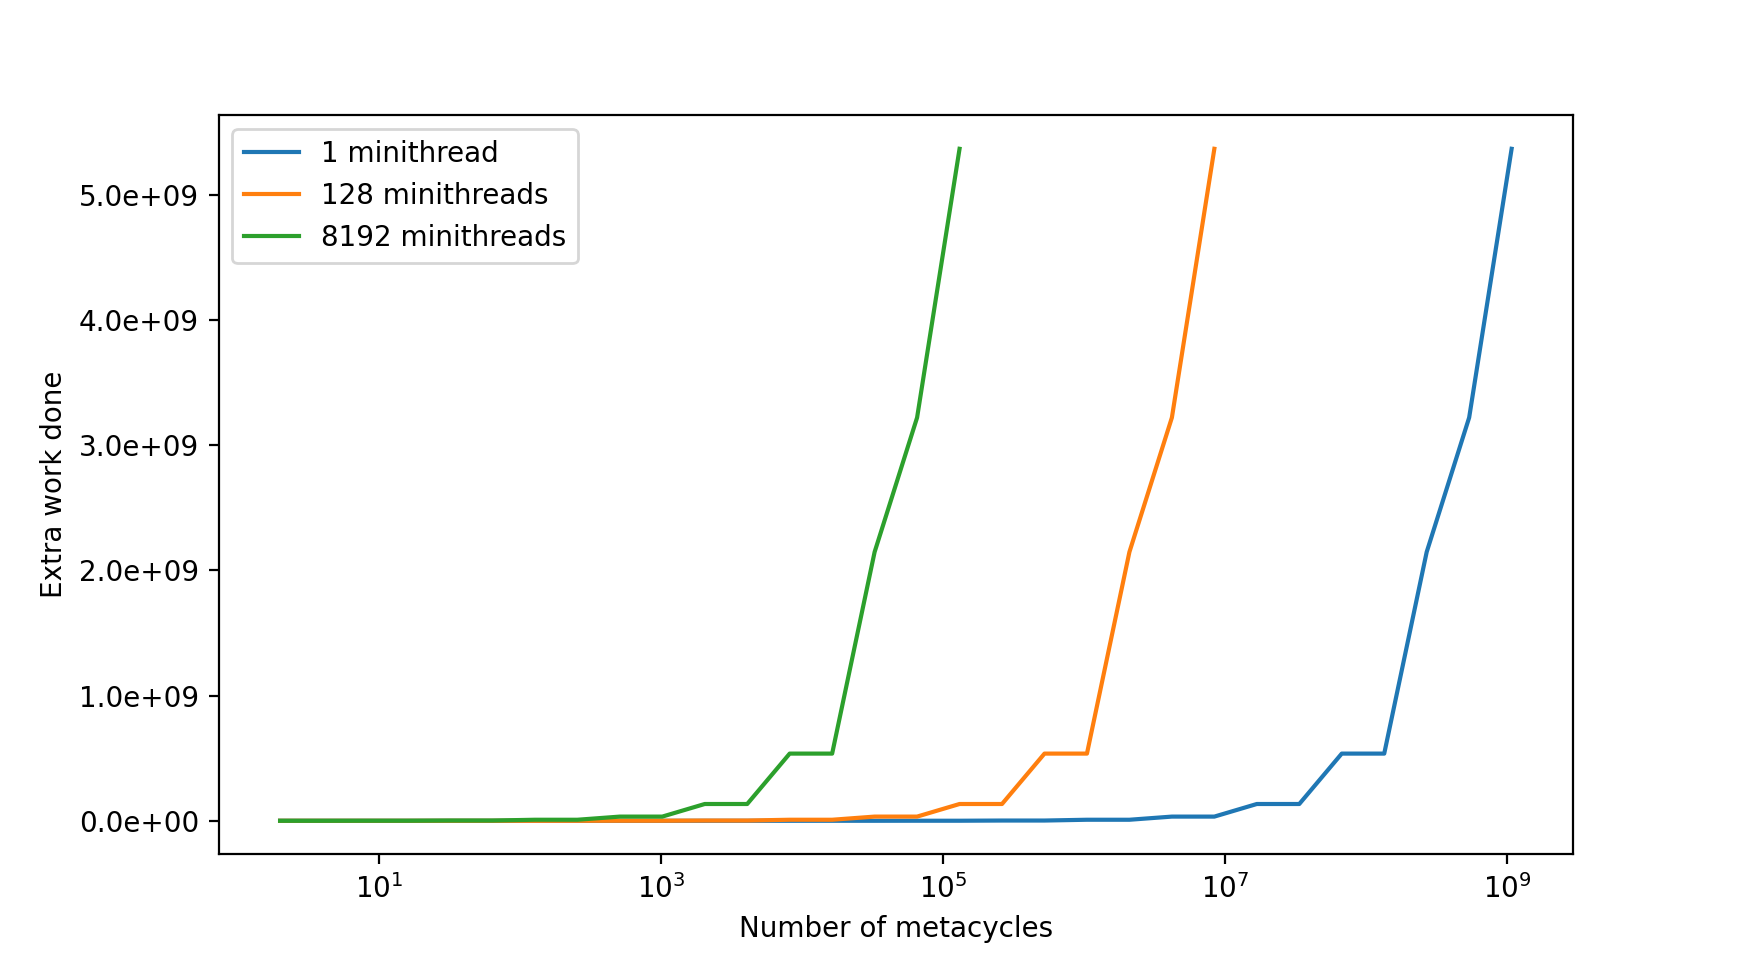
\includegraphics[width =1\textwidth]{images/teste2_work_fixaxis.png}
    \caption{Amount of extra work done by each configuration of minithreads when trying to run a constant amount of work ($2^{30}$) over certain metacycles}
    \label{work_done}
\end{figure}

As we suspected figure \ref{work_done} shows that at low number of cycles per metacycles we are 6 x\textquotesingle ing the amount of work that was asked for, inflating the time of execution.
 
\subsection{Fixing overwork} \label{fixing overwork}
To stop our minithreads of doing overwork we matched each minithread to a variable that keeps track of the work done by that minithread, we can take the work asked to the system and divide it with the number of minithreads getting the work expected to be done by a single minithread, when the variable of a minithread exceeds this number we stop executing it for the rest of metacycles as it has done all the work asked.

This method still leaves some overwork proportional to the number of minithreads running and the resolution on the instrumentation but it is now orders of magnitude smaller than the work asked to perform so we can ignore it.

With our overwork problem solved we ran again the same benchmark but we didn\textquotesingle t include the results for branch optimized instrumentation as it would double the time it took to gather the data and from the last results it was evident that would not change only by removing extra work as it doesn\textquotesingle t change the number of context switches.
 \begin{figure}[hbt]
     \centering
     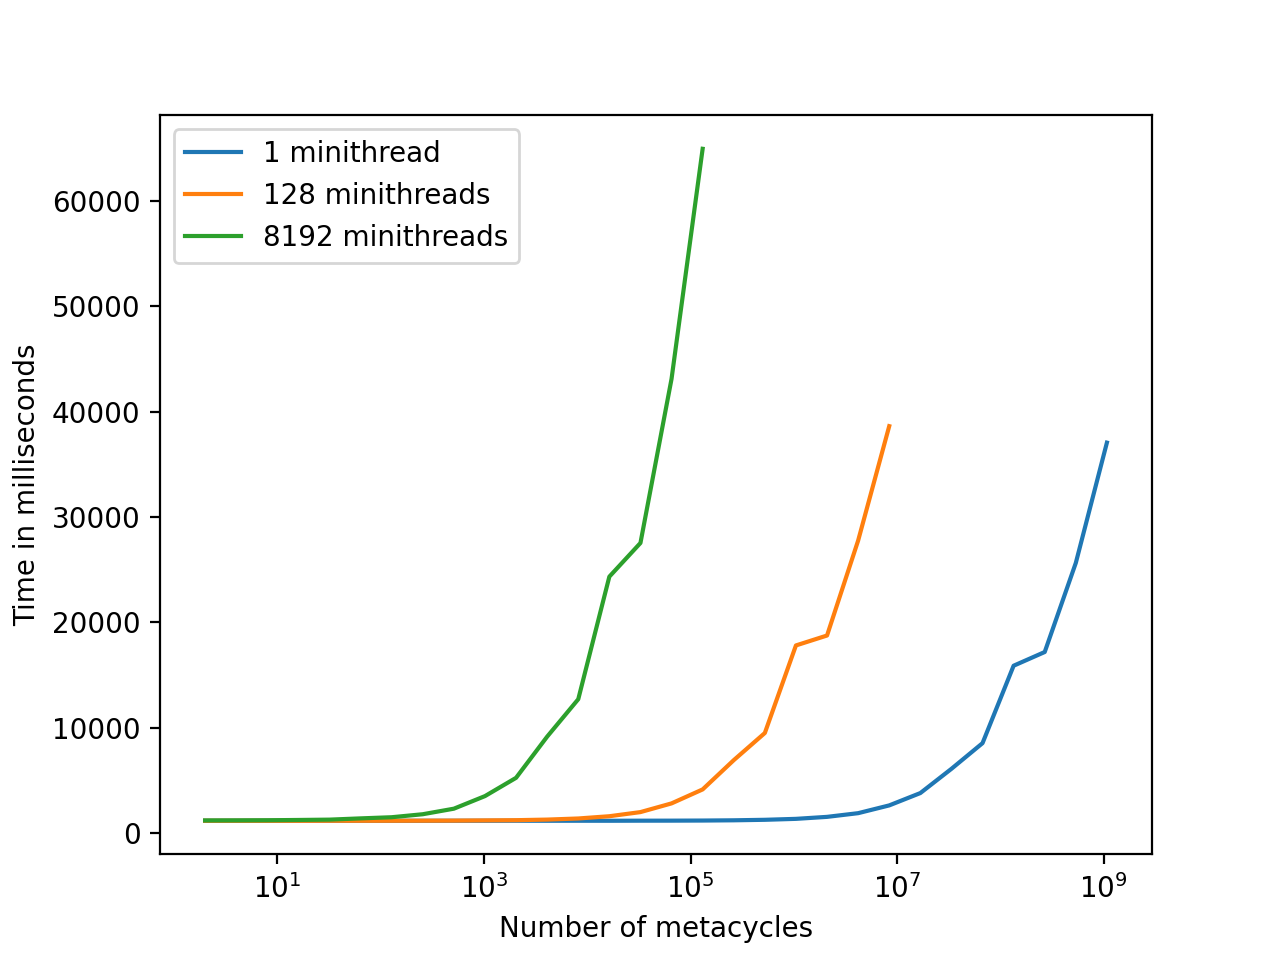
\includegraphics[width =0.7\textwidth]{images/teste5_context_switch_fixed2_bin.png}
     \caption{Time to execute a constant amount of work ($2^{30}$) for different amounts do metacycles corrected for overwork}
     \label{context_switch_fixec}
 \end{figure}
As predicted (figure \ref{context_switch_fixec}) the extra work had impact on the performance lowering the time to 1 6th, in line with the finding on figure \ref{cache_threads}.

\subsection{Side effects of fixing overwork}
Our skip method has one flaw when trying to measure the number of cycles that a context switch takes. Because we are skipping context switches when a minithread as done its expected work \ref{fixing overwork}, the actual number of context switched done is much lower.

By analyzing our fix for all the setups we got the number of context switches skipped (figure \ref{cycles skiped}):

\begin{figure}[hbt]
    \centering
    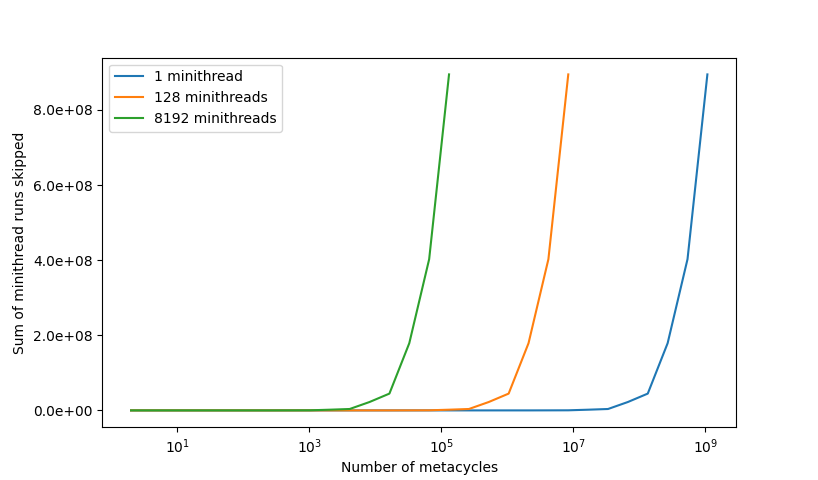
\includegraphics[width =0.85\textwidth]{images/teste3_cycles_skipped2_fixaxis.png}
    \caption{Sum of runs skipped for each configuration of minithreads for low numbers of cycles per metacycles for $2^{30}$ of work}
    \label{cycles skiped}
\end{figure}

This data (figure \ref{cycles skiped}) can be also used to approximate the resolution that gcctally was capable of instrumenting. by dividing the number of context switches that was supposed to run and the real number when doing 1 cycle per metacyles we find the average size of a basic\_block for the random\_walk function used, $\sim$ 6 cycles per basic\_block, witch corresponds to doing 6 times the work when trying to do 1 cycle per metacycle without correction.
\subsection{Findings}
Now with all the corrections done we can finally calculate the cost of doing a context switch.

First we did a visual estimate of the cost by instrumenting our run function and locking at the assembly code produced as adding up all the tally sub instructions. This plus the macros to save and restore registers gave us a base line of 265 cycles. \\
With this we can assume that our context switch is between 100 and 1000 cycles.

We also need a base line time of the function running without context switched. We can get this by averaging the times on figure \ref{context_switch_fixec} for 1 minithread for the first couple of data points as the cost of context switching up to 32 times is insignificant based on our estimate for its cycles.

This gets us a time of 1165 milliseconds to perform $2^{30}$ cycles of work in 1 and 128 minithreads and 1213 for 8192 minithreads.

Examining the data points were the number of cycles per metacycles is low enough that the context switch cost has an impact, when each minithread is performing 1024 cycles or less per metacycle, we can determine the time cost for a context switch with this formula: 

\begin{equation}
    \frac{t - 1175}{c}
\end{equation}

where $t$ is the time taken to perform the work and $c$ the number of context switches performed.

By averaging the results for each setup of minithreads we get this result (table \ref{cost_context_switch}).

\begin{table}[]
\begin{tabular}{llll}
Num. of minithreads & 1      & 128    & 8192   \\ \hline
Milliseconds per cycle & 1.08e-6 & 1.88e-6 & 1.12e-6 \\
Milliseconds per context switch      & 3.85e-4 & 4.0e-4 & 4.99e-4 \\ 
Cycles per context switch & 355 & 375 & 441
\end{tabular}
\caption{Cost in milliseconds of a context switch for some configuration of minithreads}
\label{cost_context_switch}
\end{table}

By knowing the time that it takes to perform a context switch and knowing that $2^{30}$ cycles takes 1165 milliseconds we can determine how many cycles it takes to perform a context switch (table \ref{cost_context_switch}), we can justify the different in costs for the different configurations by the performance hit examine by running multiple minithreads (figure \ref{cache_threads}).
% -----------------------------------------------------------------------------
% End inlined source: ch4.tex
% -----------------------------------------------------------------------------
\clearpage
\clearpage
% -----------------------------------------------------------------------------
% Begin inlined source: ch5.tex
% -----------------------------------------------------------------------------
\chapter{Conclusion}
\section{Evaluating the library performance}
So how good is the Tally library? We think that there are to main factors to consider when evaluating it.
\begin{itemize}

    \item Fairness
    Fairness is how precise the actual instrumentation process can represent the actual cycles executed by the each function.
    
    Because we use the same model to estimate every instrumented function it is reasonable to assume that the cost for the same kind of instruction in one instrumented function is the same as in another instrumented function.
    
    This cost might not be a true representation of the number of cycles used by this instructions (as discussed in \ref{instrumentation estimate} the instrumentation can only estimate the CPU cycle cost of each instruction) but it is a linear estimate of the value consistent throughout every instrumentation done.  
    
    \item Granularity
    
    This is how fine-grain can we go on the number of cycles asked to be ran by a minithread.
    
    The granularity is given by two factors, the average cycle cost of a basic block, (this was one of the problems encountered when trying to measure the second factor of granularity, see \ref{overwork} ) and the cost of each context switch.
    
    The average cycle cost can depend on the type of code we instrument, during our testing we found a average cost of 6 cycles when running the random walk, a simple and short function but when testing with some Competitive programming solutions (where code is highly linear) we found  18-22 cycles of average cost of basic block (this was done by visual inspection of the resulting assembly code).
    
    We found the cost of a context switch to be 350-450 cycles (table \ref{cost_context_switch}) depending on the number of minithreads ruining. 
    
    All this means that except with highly linear code the major factor determining the granularity of the library is the context switch. One of the things that can help lower this cost and elevate the granularity is to not support float operations as not only this adds a lot of instructions to save this registers but also the instructions needed are a lot slower when comparing to accessing normal registers. 
    
    The maximum granularity that this library can achieve on the current state is of about 1500 cycles (counting the cost of the context switch) without beginning to be affected by issues like overwork of the performance hit of performing the context switches.
\end{itemize}

In the end we found that the current implementation of this library meets the expectations. Although the granularity is not as fine as desired, the library can support a large amount of concurrent instrumented programs with a very small overhead (section \ref{multi thread pref hit}) when respecting its granularity. The cache performance of the library is also very predictable helping estimating performances without ever needing to run simulations.

\section{Future work}
During the execution of the project some ideas were raised but because of the time constrained were in the end left for future expansions.
\subsection{A better estimator of CPU cycles cost}
As we noted the GIMPLE representation is not the best to estimate the number of assembly instructions present on a linear block of code.

The next step is to build our own control-flow graph from the assembly code produced by a normal compilation. This way we have the exact amount of instructions performed. 

Out new instrumentation plugin would insert code on this assembly code directly before finishing the compilation.

\subsection{Overwork manager}
As one of the bigger issues with our library is the overwork performed when trying to run less cycles than our granularity permits. One of the ways of fixing this when running multiple times the same minithread is to implement a system that over time does not let the minithread execute during multiple runs so it can compensate all the extra work done on previous runs.

\subsection{Multi threading}
One of the bets ways of raising performance is to use more cores. Implementing an thread manager capable of executing multiple minithreads at the same time on different cores is one of the ultimate goals of the library. None of the implementation decisions made until now prevents this from happening. 

\subsection{Compatibility with other languages ans compilers}
Although we show this library being used in Gcc with C code, the libraries goal is to be able to instrument all compiled languages. Writing a plugin works with LLVM inserting the same mechanisms on would be a great step forwards.

\section{Auto evaluation}
This was my first experience not only doing a bigger sized project but also writing a library for other people to use. Throughout the project i learned new technologies like using Cmake for staged compilation or debugging registers and context switches with sanitizer flags and GDB. 

I also consolidated a lot of knowledge gathered during my 3 years in this course, from operating system's and CPU architecture to data analysis and software architecture and of course gaining a lot more experience writing C code.  

The project was challenging but the final product was rewarding, to my knowledge this type of CPU scheduling was never been done. I also achieve a lot of the proposed goal ending up with a library capable of running tens of thousands of minithreads with a low overhead.
% -----------------------------------------------------------------------------
% End inlined source: ch5.tex
% -----------------------------------------------------------------------------
\clearpage
\appendix
\clearpage
% -----------------------------------------------------------------------------
% Begin inlined source: app1.tex
% -----------------------------------------------------------------------------
% \chapter{Acr\'onimos}

% (Opcional...)


\chapter{Code}
\begin{lstlisting}[language=C,style=CStyle,caption=Context switch excerpt, label = {context code}, escapechar=|]
    _thread_sp = thread->sp;

run    PUSH_REGISTERS; 

    asm volatile("\tmovq %%rsp, %0\n" : "=m" (_my_sp) ); 
    asm volatile("\tmovq %0, %%rsp\n" : : "m" (_thread_sp) );

    if (thread->state == MINITHREAD_NEW) {
        thread->state = MINITHREAD_RUNNING;
        (thread->body)->fptr(thread->init_Args); |\label{call func}|
    }else {
        thread->state = MINITHREAD_RUNNING;

        POP_REGISTERS; |\label{pop regs}|

        asm volatile("\tret\n"); |\label{ret instr}|
    }

    asm (
        "_minithread_break:\n" |\label{minithread break label}|
    );

    PUSH_REGISTERS; |\label{push regs}|

    asm volatile("\tmovq %%rsp, %0\n" : "=m" (_thread_sp) : ); |\label{save sp}|
    asm volatile("\tmovq %0, %%rsp\n" : : "m" (_my_sp) );   |\label{put sp}|

    POP_REGISTERS;

    thread->sp = _thread_sp;

\end{lstlisting}

\begin{lstlisting}[language=C,style=CStyle,caption=Context switch macros, label = {context macros}]
    #define PUSH_REGISTERS asm (\
    "\tpushq %r14\n"\
    "\tpushq %r13\n"\
    "\tpushq %r12\n"\
    "\tpushq %r11\n"\
    "\tpushq %r10\n"\
    "\tpushq %r9\n"\
    "\tpushq %r8\n"\
    "\tpushq %rbp\n"\
    "\tpushq %rdi\n"\
    "\tpushq %rsi\n"\
    "\tpushq %rbx\n"\
    "\tpushq %rdx\n"\
    "\tpushq %rcx\n"\
    "\tpushq %rax\n"\
    "\tsub $128, %rsp\n" /* 16 (8 * 2) (128 bit per float register) * 8 */  \
    "\tmovhps %xmm0, -128(%rsp)\n"\
    "\tmovlps %xmm0, -120(%rsp)\n"\
    "\tmovhps %xmm1, -112(%rsp)\n"\
    "\tmovlps %xmm1, -104(%rsp)\n"\
    "\tmovhps %xmm2, -96(%rsp)\n"\
    "\tmovlps %xmm2, -88(%rsp)\n"\
    "\tmovhps %xmm3, -80(%rsp)\n"\
    "\tmovlps %xmm3, -72(%rsp)\n"\
    "\tmovhps %xmm4, -64(%rsp)\n"\
    "\tmovlps %xmm4, -56(%rsp)\n"\
    "\tmovhps %xmm5, -48(%rsp)\n"\
    "\tmovlps %xmm5, -40(%rsp)\n"\
    "\tmovhps %xmm6, -32(%rsp)\n"\
    "\tmovlps %xmm6, -24(%rsp)\n"\
    "\tmovhps %xmm7, -16(%rsp)\n"\
    "\tmovlps %xmm7, -8(%rsp)\n"\ 
    );
    
    #define POP_REGISTERS asm (\
    "\tadd $128, %rsp\n" /* 16 (8 * 2) (128 bit per float register) * 8 */  \
    "\tmovhps %xmm0, -128(%rsp)\n"\
    "\tmovlps %xmm0, -120(%rsp)\n"\
    "\tmovhps %xmm1, -112(%rsp)\n"\
    "\tmovlps %xmm1, -104(%rsp)\n"\
    "\tmovhps %xmm2, -96(%rsp)\n"\
    "\tmovlps %xmm2, -88(%rsp)\n"\
    "\tmovhps %xmm3, -80(%rsp)\n"\
    "\tmovlps %xmm3, -72(%rsp)\n"\
    "\tmovhps %xmm4, -64(%rsp)\n"\
    "\tmovlps %xmm4, -56(%rsp)\n"\
    "\tmovhps %xmm5, -48(%rsp)\n"\
    "\tmovlps %xmm5, -40(%rsp)\n"\
    "\tmovhps %xmm6, -32(%rsp)\n"\
    "\tmovlps %xmm6, -24(%rsp)\n"\
    "\tmovhps %xmm7, -16(%rsp)\n"\
    "\tmovlps %xmm7, -8(%rsp)\n"\ 
    "\tpopq %rax\n"\
    "\tpopq %rcx\n"\
    "\tpopq %rdx\n"\
    "\tpopq %rbx\n"\
    "\tpopq %rsi\n"\
    "\tpopq %rdi\n"\
    "\tpopq %rbp\n"\
    "\tpopq %r8\n"\
    "\tpopq %r9\n"\
    "\tpopq %r10\n"\
    "\tpopq %r11\n"\
    "\tpopq %r12\n"\
    "\tpopq %r13\n"\
    "\tpopq %r14\n"\
    );
\end{lstlisting}
\newpage
\begin{lstlisting}[language=C,style=CStyle,caption=Minithread structure,label={minithread struct}] 
struct stMinithread {
    /// stack-pointer for the minithread
    void **sp;
    
    ///usefull for cheking how much memory is in use (bottom of the stack) 
    void **sp_base;   
    
    /// position of memory allocated for the stack (which happens to be the top of the stack)
    void **stack;

    /// last position of memory usesd by modules, this means that sp can go from stack to stack top - 1
    void **stack_top;

    //paramm given to the initial function
    void* init_Args;

    /// ammount of memory allocated for the stack (in terms of sizeof(void*)-long words)    
    uint64_t memory_size_bytes;
    
    /// whether the thread is currently stopped, running, paused or interrupted
    MinithreadState state;
    
    /// the function to be run when the thread starts
    MinithreadCode body;

    //amount of cycles needed to run, this number does not change during execution of the thread
    uint64_t cycles_to_run;
    //amount of cycles left when execution is stopped
    uint64_t cycles_left;

    //array of modules all malloced, shoud be sorted by name hash
    MinithreadModules *modules;

};
\end{lstlisting}

\begin{lstlisting}[language={[x86masm]Assembler}, basicstyle=\small, caption=decrease tally from the register r15]
    sub     basic_block size, $r15
\end{lstlisting}  
\begin{lstlisting}[language={[x86masm]Assembler}, basicstyle=\small, caption=decrease tally from the C variable counter]
    pushq   $r15
    pushq   $rdx
    movq    counter@GOTPCREL(%rip), %r15
    movq    (%r15), %r15
    sub	    basic_block size, %r15
    movq    counter@GOTPCREL(%rip), %rdx
    movq    %r15, (%rdx)
    popq    $rdx
    popq    $r15
     
\end{lstlisting}
% -----------------------------------------------------------------------------
% End inlined source: app1.tex
% -----------------------------------------------------------------------------
\clearpage
\renewcommand{\bibname}{References}
\addcontentsline{toc}{chapter}{References}
\bibliographystyle{plain}
%\bibliography{refs}


\begin{thebibliography}{}
\bibitem[Intel® 64 and IA-32 Architectures Optimization Reference Manual]{Intel}
https://www.intel.com/content/dam/doc/manual/64-ia-32-architectures-optimization-manual.pdf

\bibitem[Stackoverflow $<$symbol$>$@GOTPCREL(\%rip) explained]{stack gotp}
https://stackoverflow.com/a/66713969

\bibitem[Gimble basic block]{gimple bb}
https://gcc.gnu.org/onlinedocs/gccint/Basic-Blocks.html

\bibitem[Wikipedia branch predictor]{bpo}
https://en.wikipedia.org/wiki/Branch\_predictor

\bibitem[Simple Heap Memory ALLocator]{SHMALL}
https://github.com/CCareaga/heap\_allocator
\end{thebibliography}
\end{document}
